\documentclass[]{article}
\usepackage[a4paper, total={6in, 10in}]{geometry}
\usepackage{hyperref}
\usepackage{amsmath}
\usepackage{graphicx}
\usepackage[outdir=./]{epstopdf}
\usepackage{booktabs}
\usepackage{float}
\usepackage{subcaption}

\setlength{\parindent}{0em}
\setlength{\parskip}{1em}

\DeclareMathOperator{\cov}{cov}

%opening
\title{SSY 230, System Identification\\
	Project 3: Identification of a Real System}
\author{Yuxuan Xia\\ \href{mailto:yuxuan.xia@chalmers.se}{yuxuan.xia@chalmers.se}\\Emil Staf\\\href{mailto:emil.staf@chalmers.se}{emil.staf@chalmers.se}}

\begin{document}

\maketitle


\section{Flexible Robot Arm}
The system we have chosen to identify is a mechanical system, where a flexible robot arm have been installed on an electrcal motor. It is a SISO system where the input $u(t)$ is measured reaction torque and the output $y(t)$ is the acceleration of the flexible robot arm. The experimental set-up was performed using a periodic sinusodial sweep.

\subsection{Data}
As mentioned previously the input data is a periodic sinusodial sweep (see top plot of Figure \ref{fig:input}). Due to the fact that the data was obtained using a periodic sinusodial sweep we split the data in half and use the first part as training data and the second part as validation data.

\begin{figure}[ht]
\centering
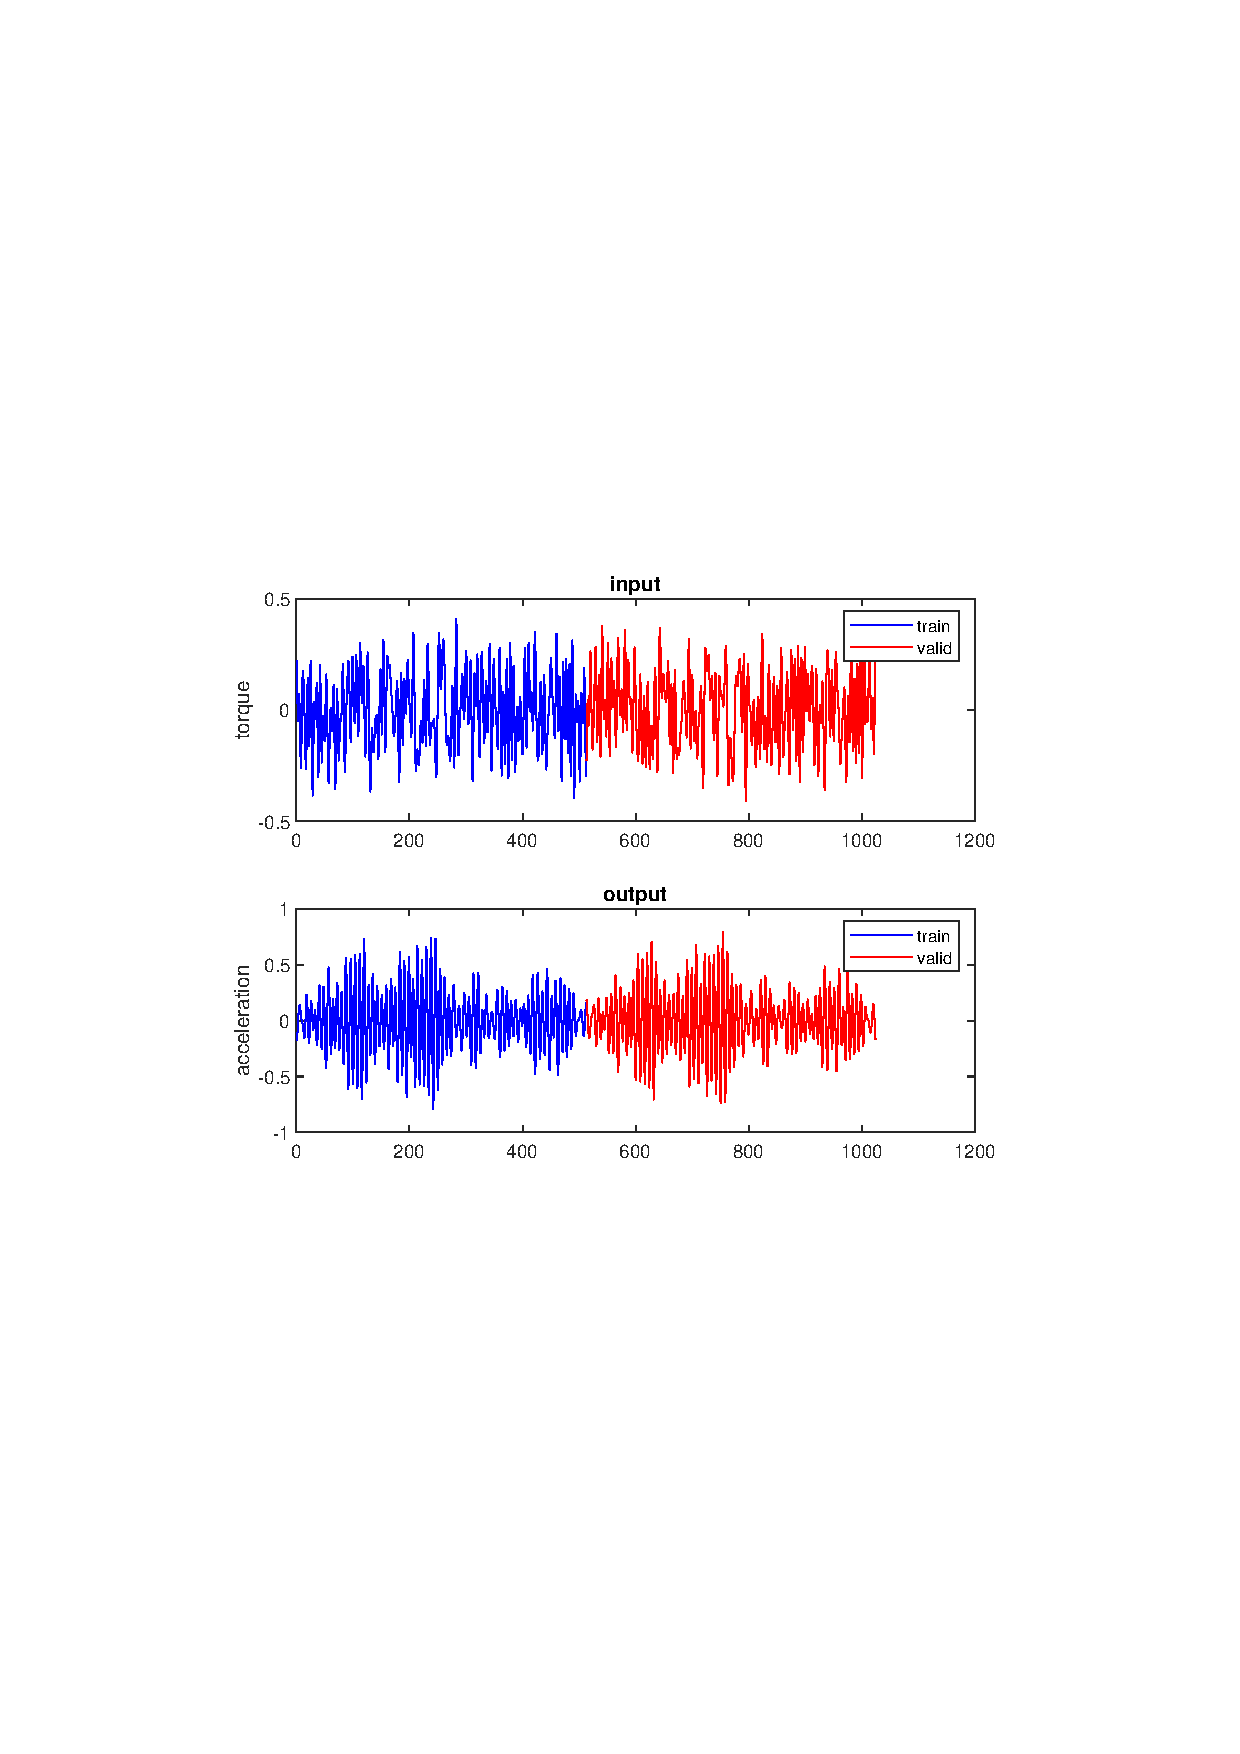
\includegraphics[trim= 10cm 8cm 10cm 8cm, scale=0.4]{figures/input.pdf}
\caption{System data, input $u(t)$ (top) and output $y(t)$ (bottom).}
\label{fig:input}

\end{figure}
To make sure that the frequency content in both the training and validation data are similar we use the \emph{etfe} in MATLAB to find the Empirical Transfer Function Estimate of training- and validation data. The resulting bode-plot is shown in Figure \ref{fig:bode-train_valid}. Because the input signal is periodic, the empirical transfer function estimate is unbiased.

\begin{figure}[ht]
\centering
\begin{subfigure}{.49\textwidth}
	\centering
	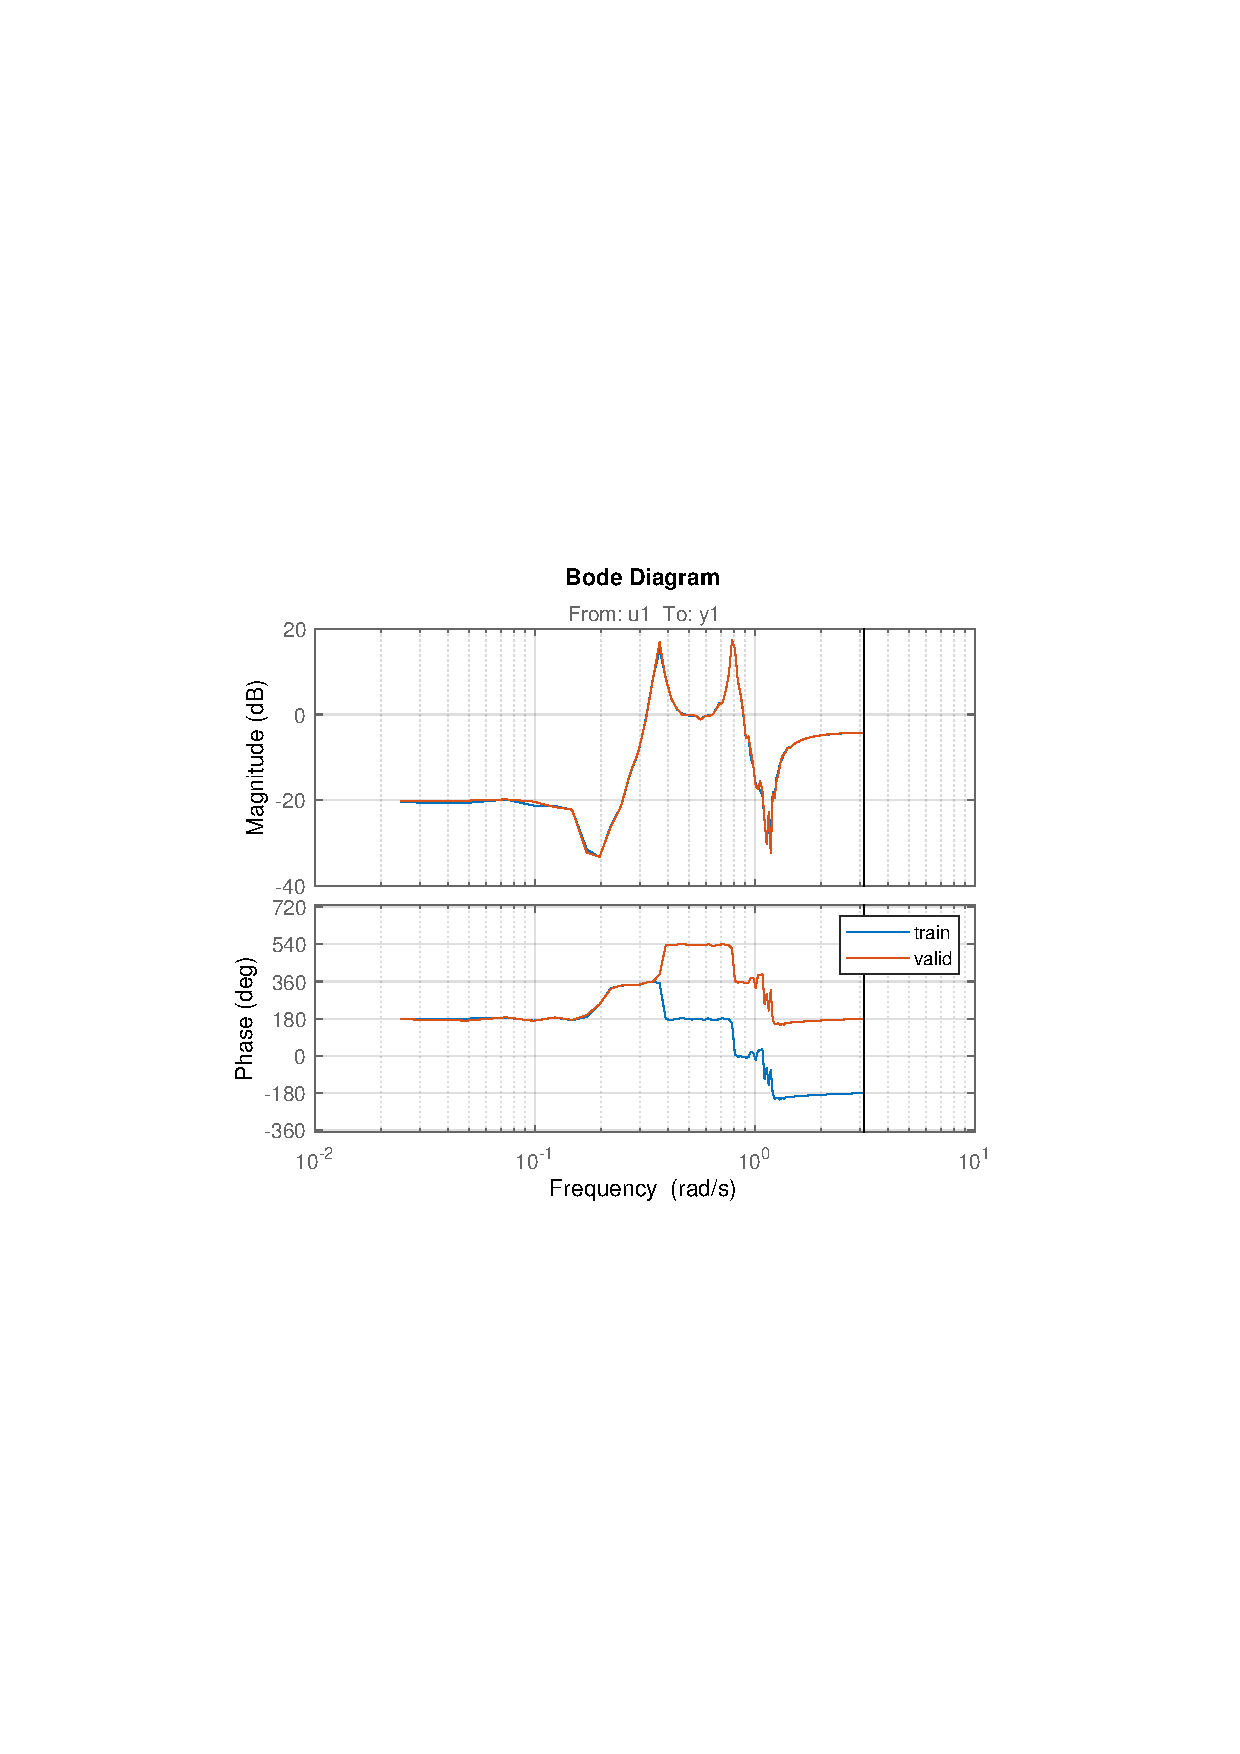
\includegraphics[trim= 10cm 8cm 10cm 8cm, scale=0.4]{figures/bode-train_valid.pdf}
	\caption{Bode-plot of training and validation data.}
	\label{fig:bode-train_valid}
\end{subfigure}
\begin{subfigure}{.49\textwidth}
	\centering
	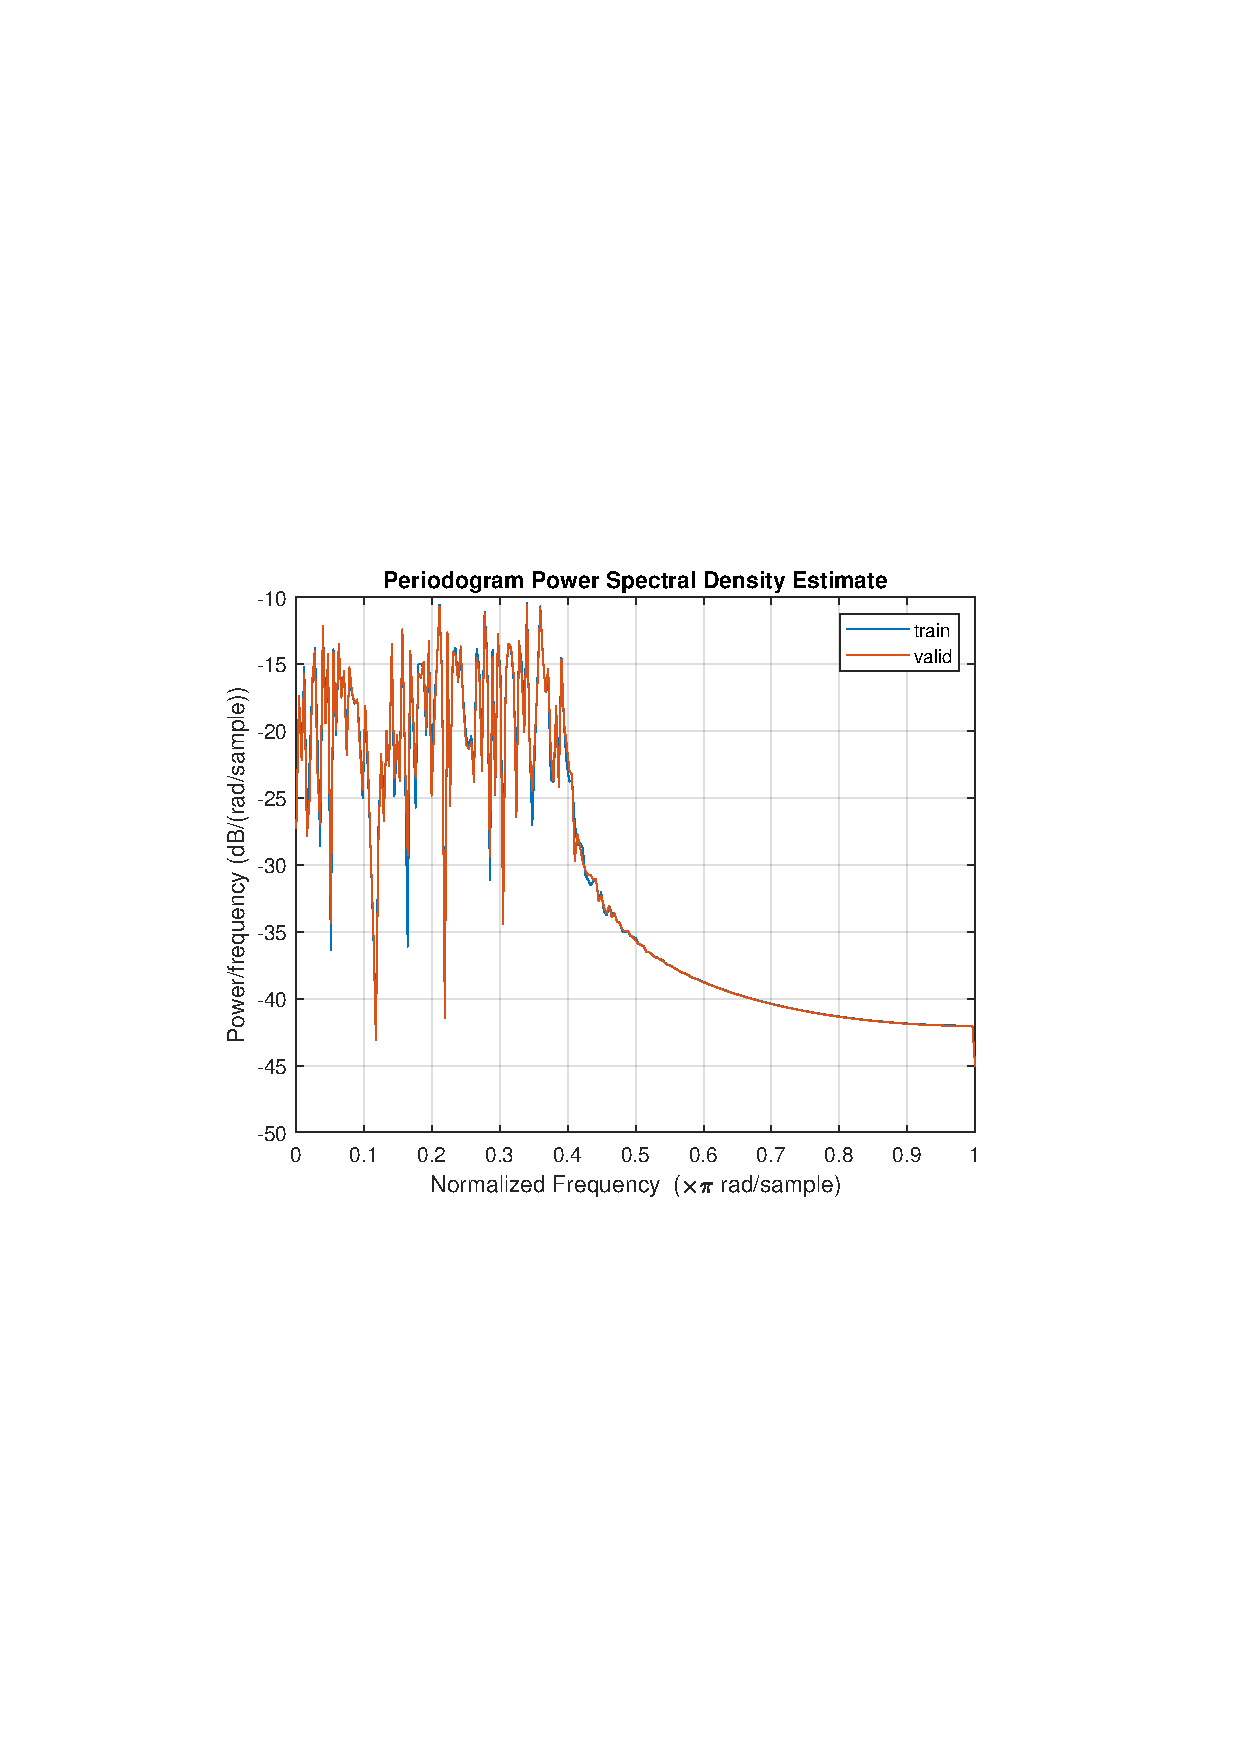
\includegraphics[trim= 10cm 8cm 10cm 8cm, scale=0.4]{figures/periodogram-train_valid.pdf}
	\caption{Periodogram of training and validation data.}
	\label{fig:periodogram-train_valid}
\end{subfigure}
\caption{Analyzing training/validation split.}
\label{fig:train_valid}
\end{figure}

From analysing Figure \ref{fig:bode-train_valid} it is clear that the amplitude of the frequency content in both training- and validation data is very similar, while there is a 360 degree phase shift approximately starting from frequencies $>0.35$ rad/s. However, it should be noted that a 360 degree phase shift means the validation data and training data are still in phase. Using the MATLAB build-in function \emph{periodogram} it is clear that the frequency content of the training- and validation data is very similar. Also, it can be seen that for frequencies $> 0.5$ rad/s the power the amount of information for each frequency decreases. By examining the bode plot, we can have an initial guess of the number of poles and zeros we can observe that there are four sharp corners, each of which represent two conjugate poles or two conjugate zeros depending on its concave or convex. The first and last parts of the amplitude plot are ladder-shaped, which means that there are two more real poles. And we can also see that there is one hollow between two spikes, which represent a zero. Thus, there are six poles and five zeros in total. The high frequency assymptote amplitude is constant, which means that (for a linear system) there should be an equal amount of poles and zeroes.

\subsection{Pre-Processing}
In off-line situations, it is often better to remove trends in data before doing the system identification so that only the dynamic features are modelled. This can be done using the \textit{getTrend} and \textit{detrend} commands in MATLAB. However, in our case, the data before and after detrending look very similar since there is no obvious trend.

\subsection{Model Estimation}
\subsubsection{Linear Models}
 In this section we search over the linear model space for candidate models. A few different linear models are tested and compared: ARX, OE, State Space and Transfer Function Estimation. 

\begin{figure}[ht]
\centering
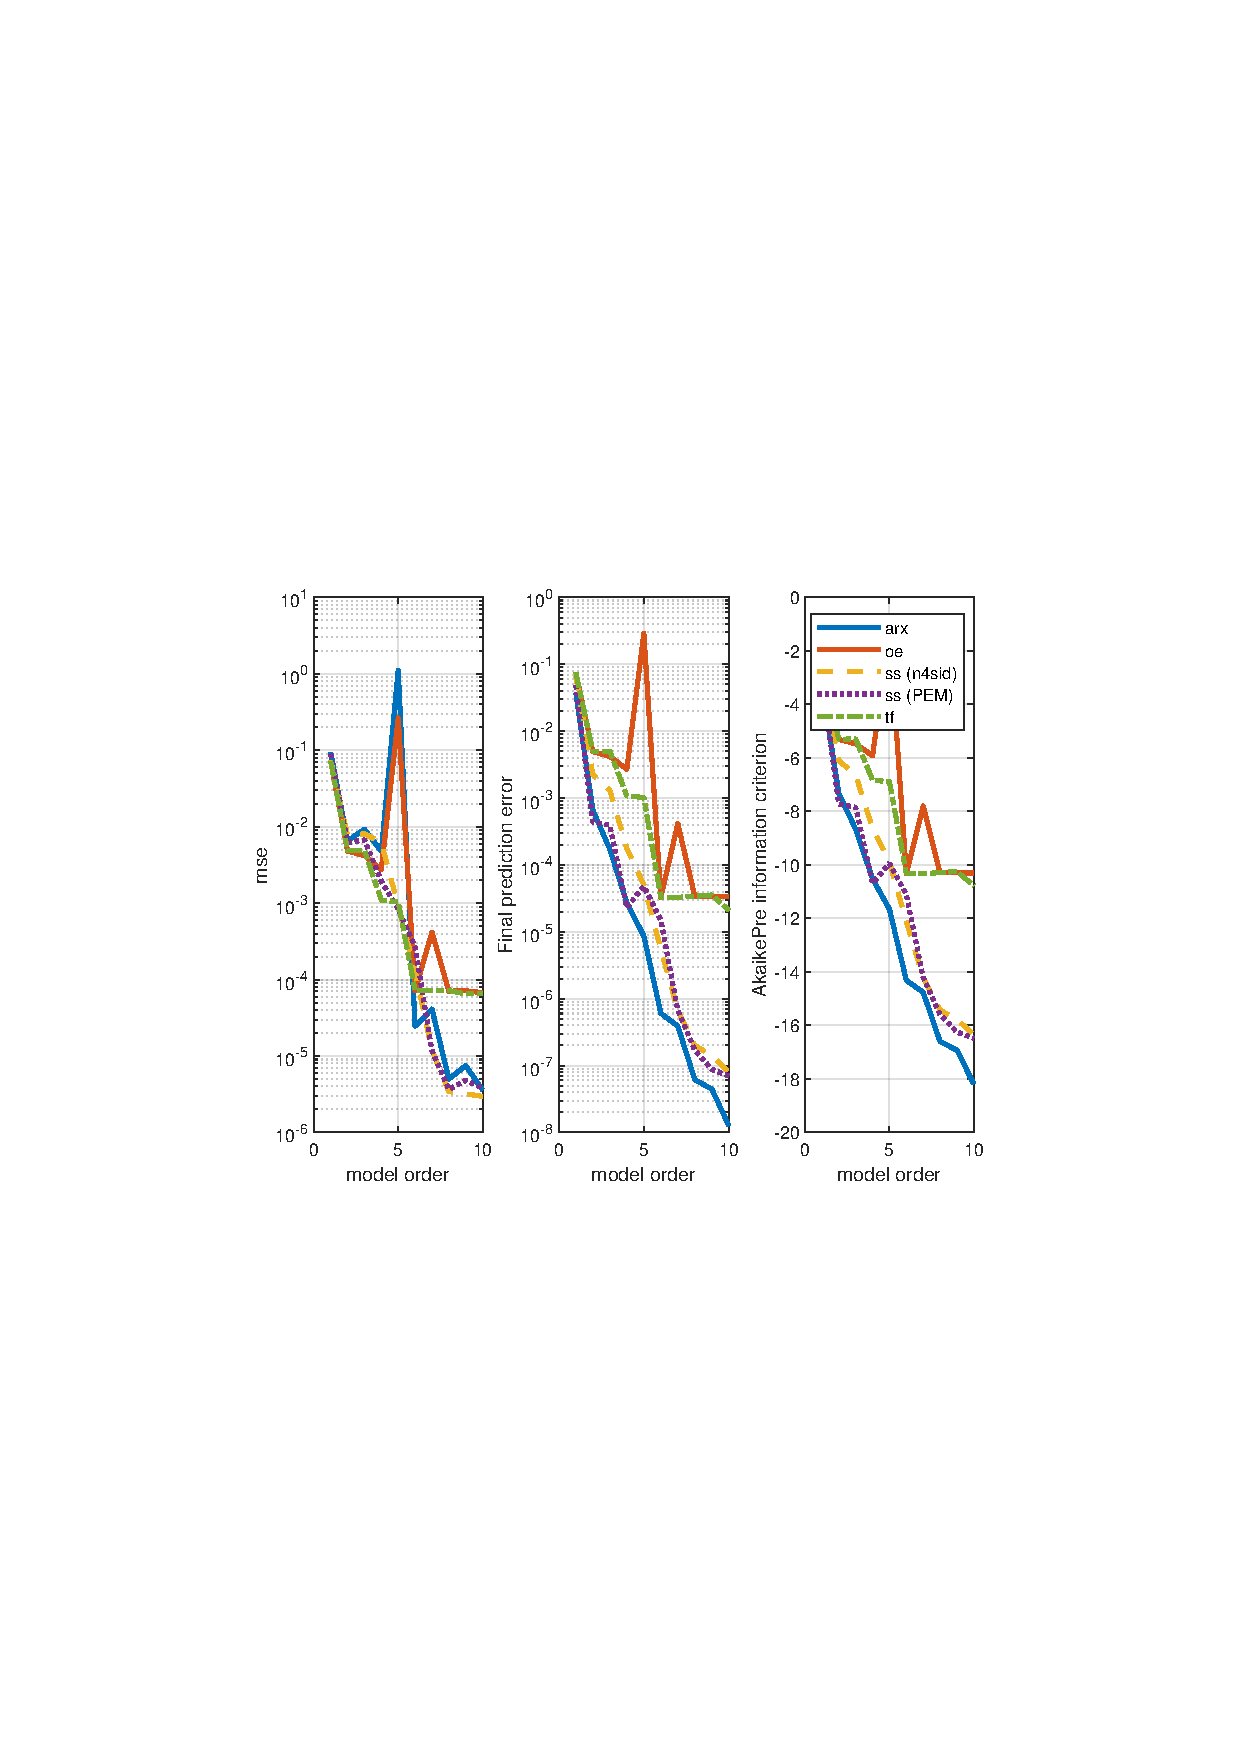
\includegraphics[trim= 10cm 8cm 10cm 8cm, scale=0.7]{figures/model_order.pdf}
\caption{Searching over different model orders $n$, where the number of parameters $p$ are $p=2n+1$.}
\label{fig:model_order}
\end{figure}
In Figure \ref{fig:model_order} the $mse$ decreases for increasing model order but start to saturate for model orders above 8. As the high frequency assymptote from the bode plot of the ETFE tells us that there should be an equal ammount of poles and zeroes, and our more specific analysis resulted in 6 poles and 5 zeroes we first try models of order 6. From Figure \ref{fig:model_order} the $mse$ shows that the models ARX, and State Space give the best results so lets focus on analysing them from now on.

\paragraph{Pole-Zero Plots}

Next, we show the pole/zero and bode plots of the ARX model and the state space model estimated using subspace method. 

The left plot in Figure \ref{fig:pzplot_arx1} shows the pole-zero map of an ARX model with model order na=nb=6, along with 95% confidence region. We can see that for the left two complex conjugate poles, there are some uncertainties. And most importantly, we can only observe 5 zeros in the plot. This is because the two zeros in the middle of the plot almost completely overlapped, which means that we can decrease one model order in the numerator of the plant model. 

Figure \ref{fig:pzplot_arx2} shows the pole/zero plot of the ARX model with model order na = 6, and nb =5. We can see that by decreasing one model order in the numerator, the uncertainties of the left two complex conjugate poles are also decreased. 

Figure \ref{fig:pzplot_ss} pole/zero plot corresponds to the state space model with order 6. Here can we can see that there is a real pole on the right half plane. This means that the system has an unstable gain. This can be also verified from this bode plot that for the state space model, the magnitude increases exponentially in the last part.  Here, we can see that the gain margin for the estimated models when phase is at -180 degree, close to the Nyquist frequency varies a lot compared to the empirical transfer function estimate, which is almost constant. This can be further verified by examining the spectral density of the data, which has very low power in high frequency part, which means for the high frequency part, not enough information is provided to give a good model estimation. 

\begin{figure}[ht]
\centering
\begin{subfigure}{.49\textwidth}
	\centering
	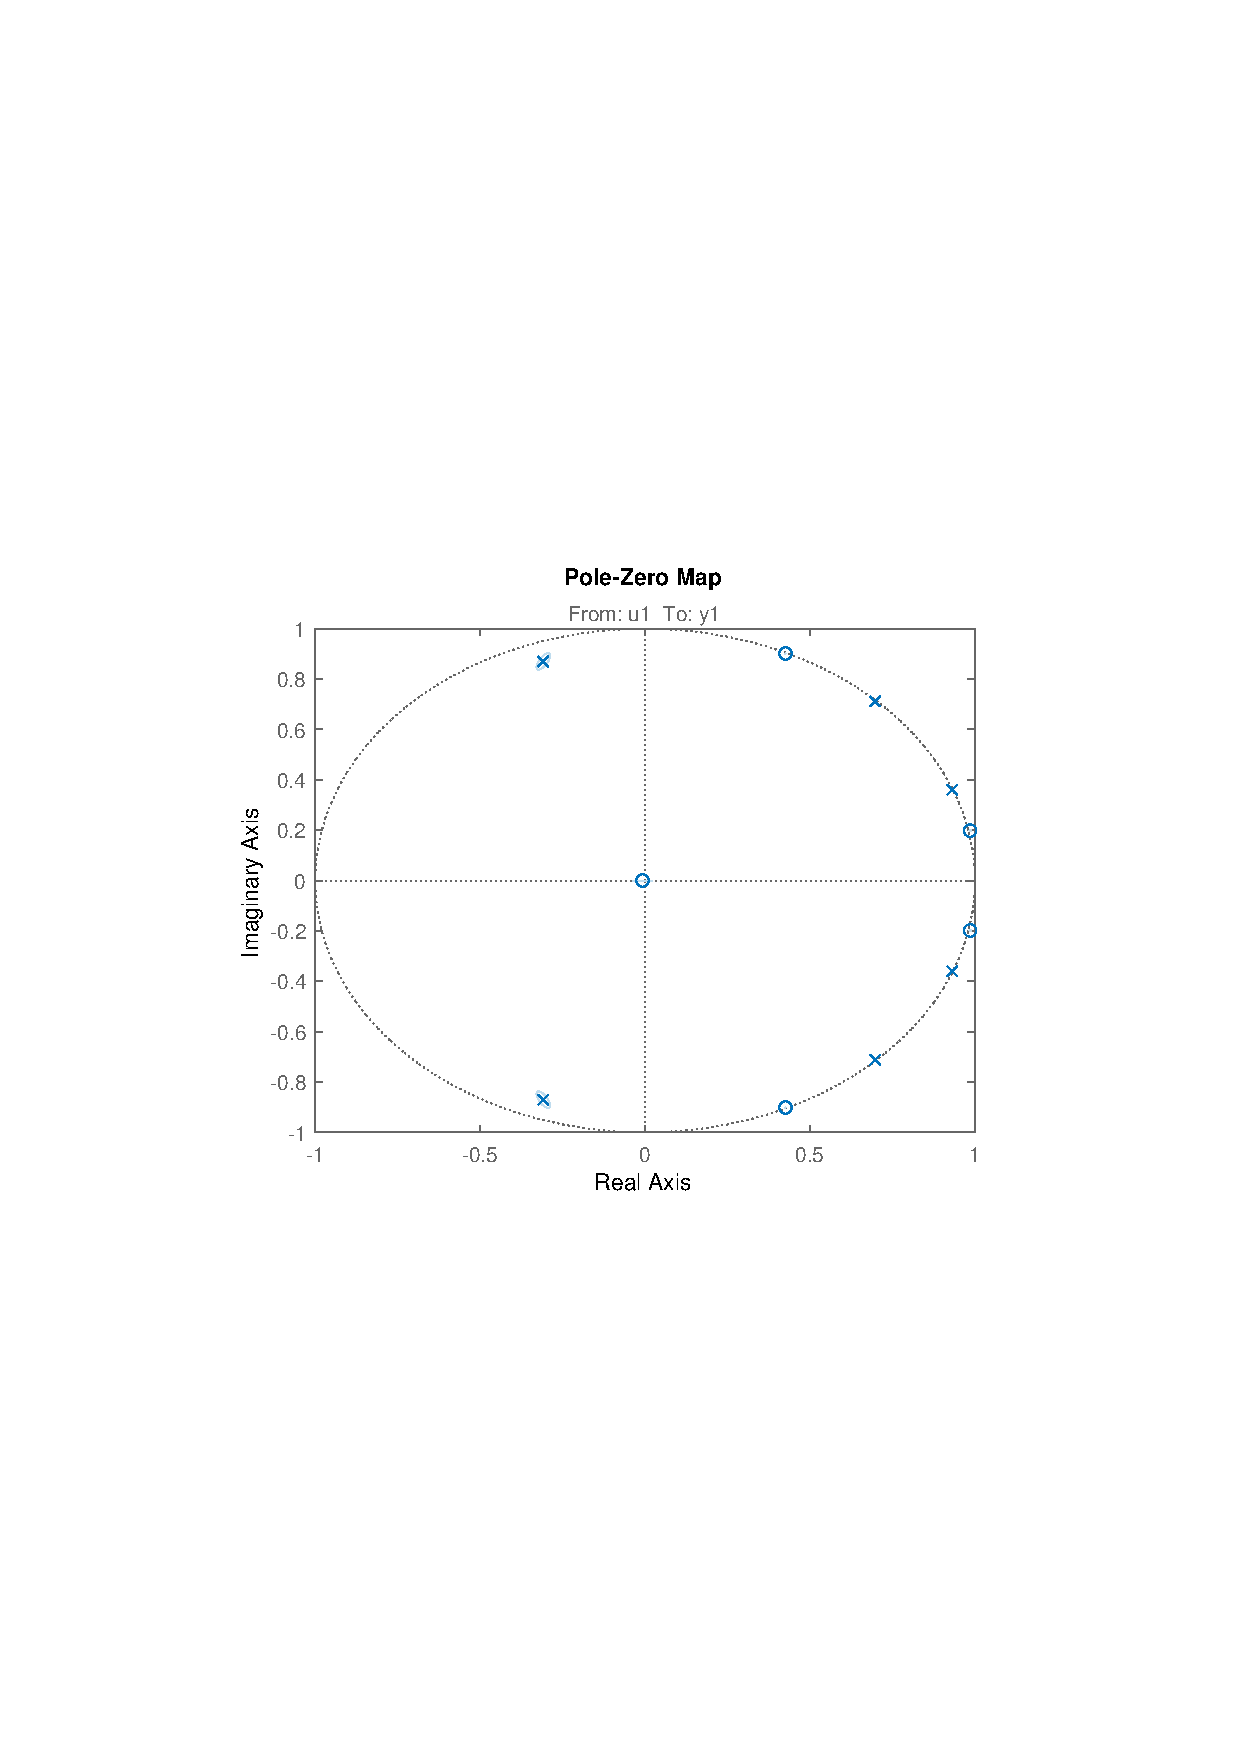
\includegraphics[trim= 10cm 8cm 10cm 8cm, scale=0.4]{figures/pz_arx_66.pdf}
	\caption{ARX na = 6 nb=6.}
	\label{fig:pzplot_arx1}
\end{subfigure}
\begin{subfigure}{.49\textwidth}
	\centering
	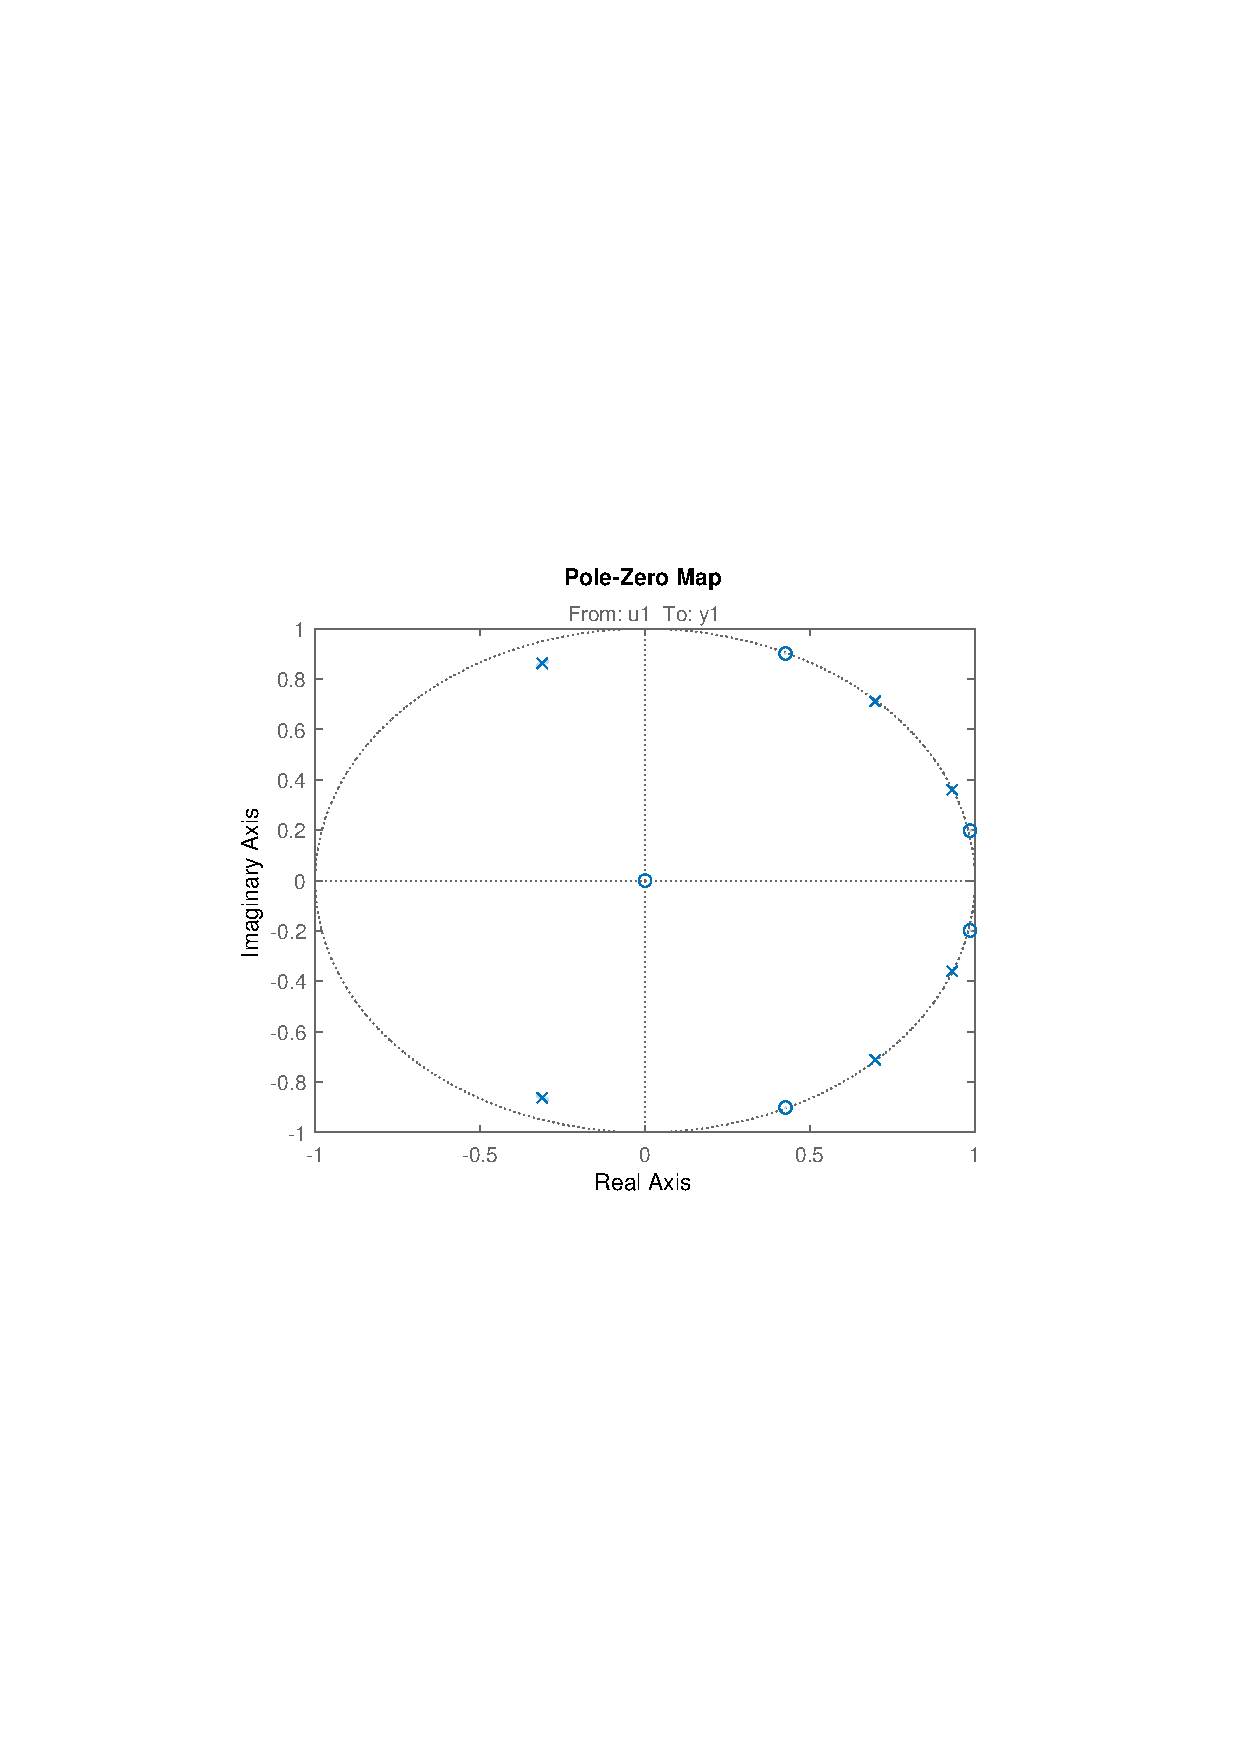
\includegraphics[trim= 10cm 8cm 10cm 8cm, scale=0.4]{figures/pz_arx_65.pdf}
	\caption{ARX na=6 nb=5.}
	\label{fig:pzplot_arx2}
\end{subfigure}
\caption{Pole/zero plots}
\label{fig:pzplot}
\end{figure}

The zero in the origin is an uncaptured time shift (positive or negative?) of the system dynamic.

\begin{figure}[ht]
\centering
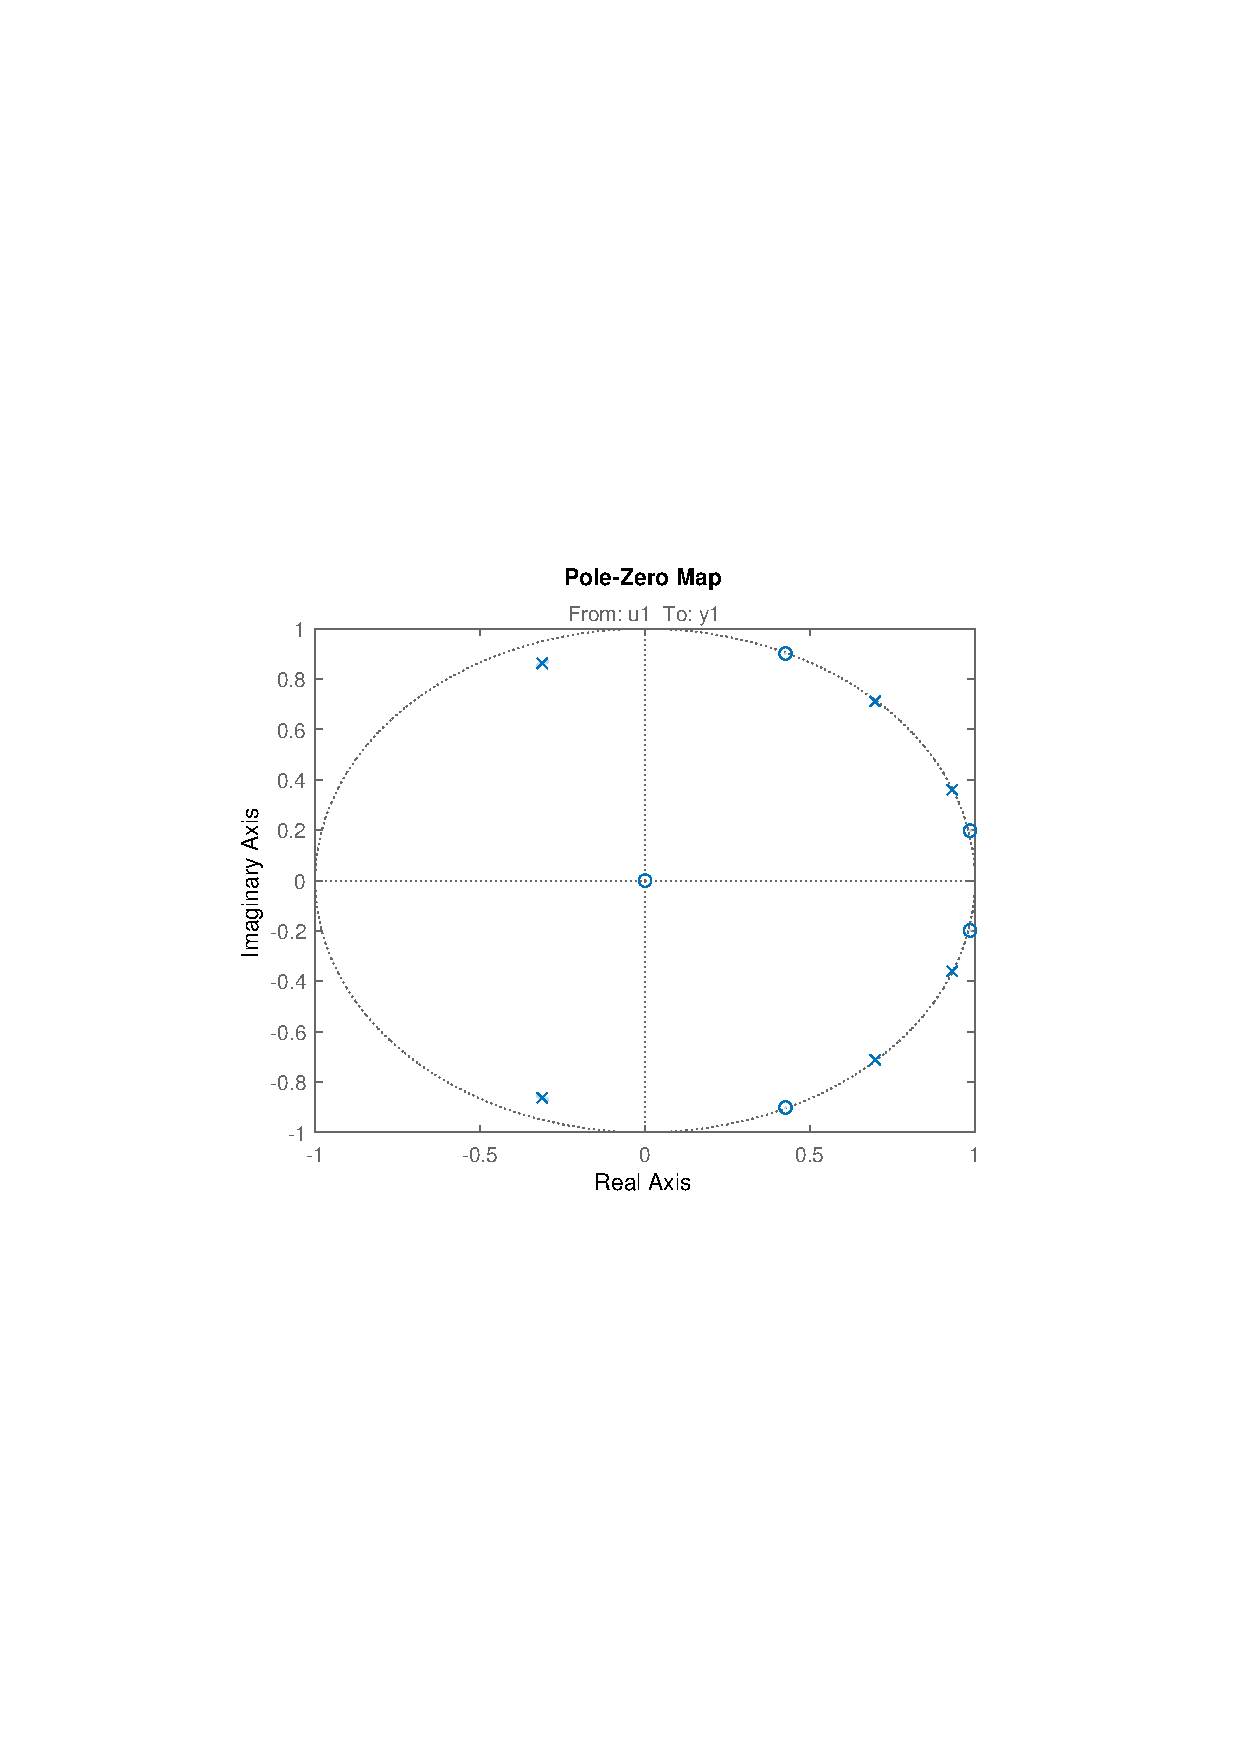
\includegraphics[trim= 10cm 8cm 10cm 8cm, scale=0.7]{figures/pz_n4sid_66.pdf}
\caption{State Space ($n4sid$).}
\label{fig:pzplot_ss}
\end{figure}

\begin{figure}[ht]
\centering
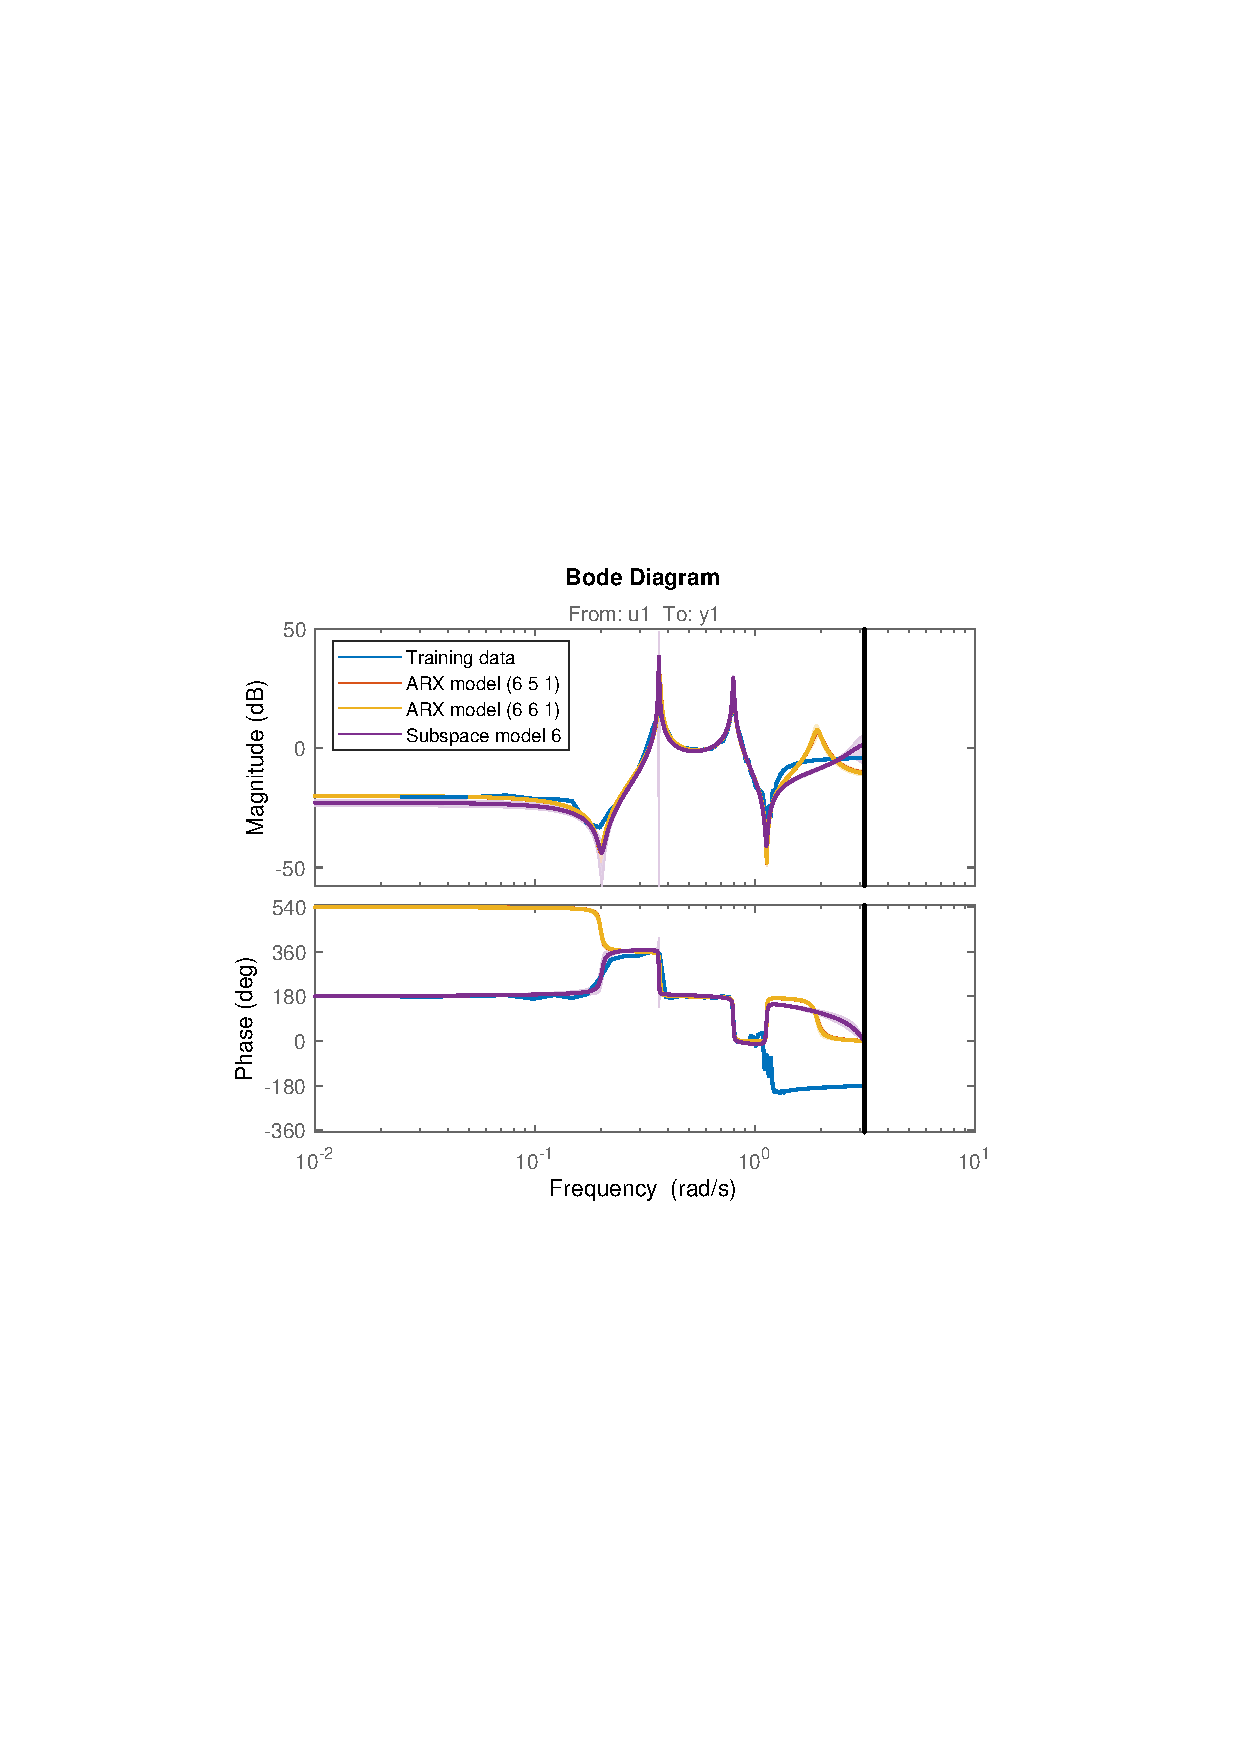
\includegraphics[trim= 10cm 8cm 10cm 8cm, scale=0.7]{figures/bode_models.pdf}
\caption{Bode plot of models.}
\label{fig:bode_models}
\end{figure}
In Figure \ref{fig:bode_models}, we can see that the gain margin when phase is at -180 degree, around the Nyquist frequency varies a lot compared to the empirical transfer function update, which is almost constant. This implies that we probability need some further data preprocessing step to filter out the high frequency component of the data.


\paragraph{Simulations}



\begin{figure}[ht]
\centering
\begin{subfigure}{.49\textwidth}
	\centering
	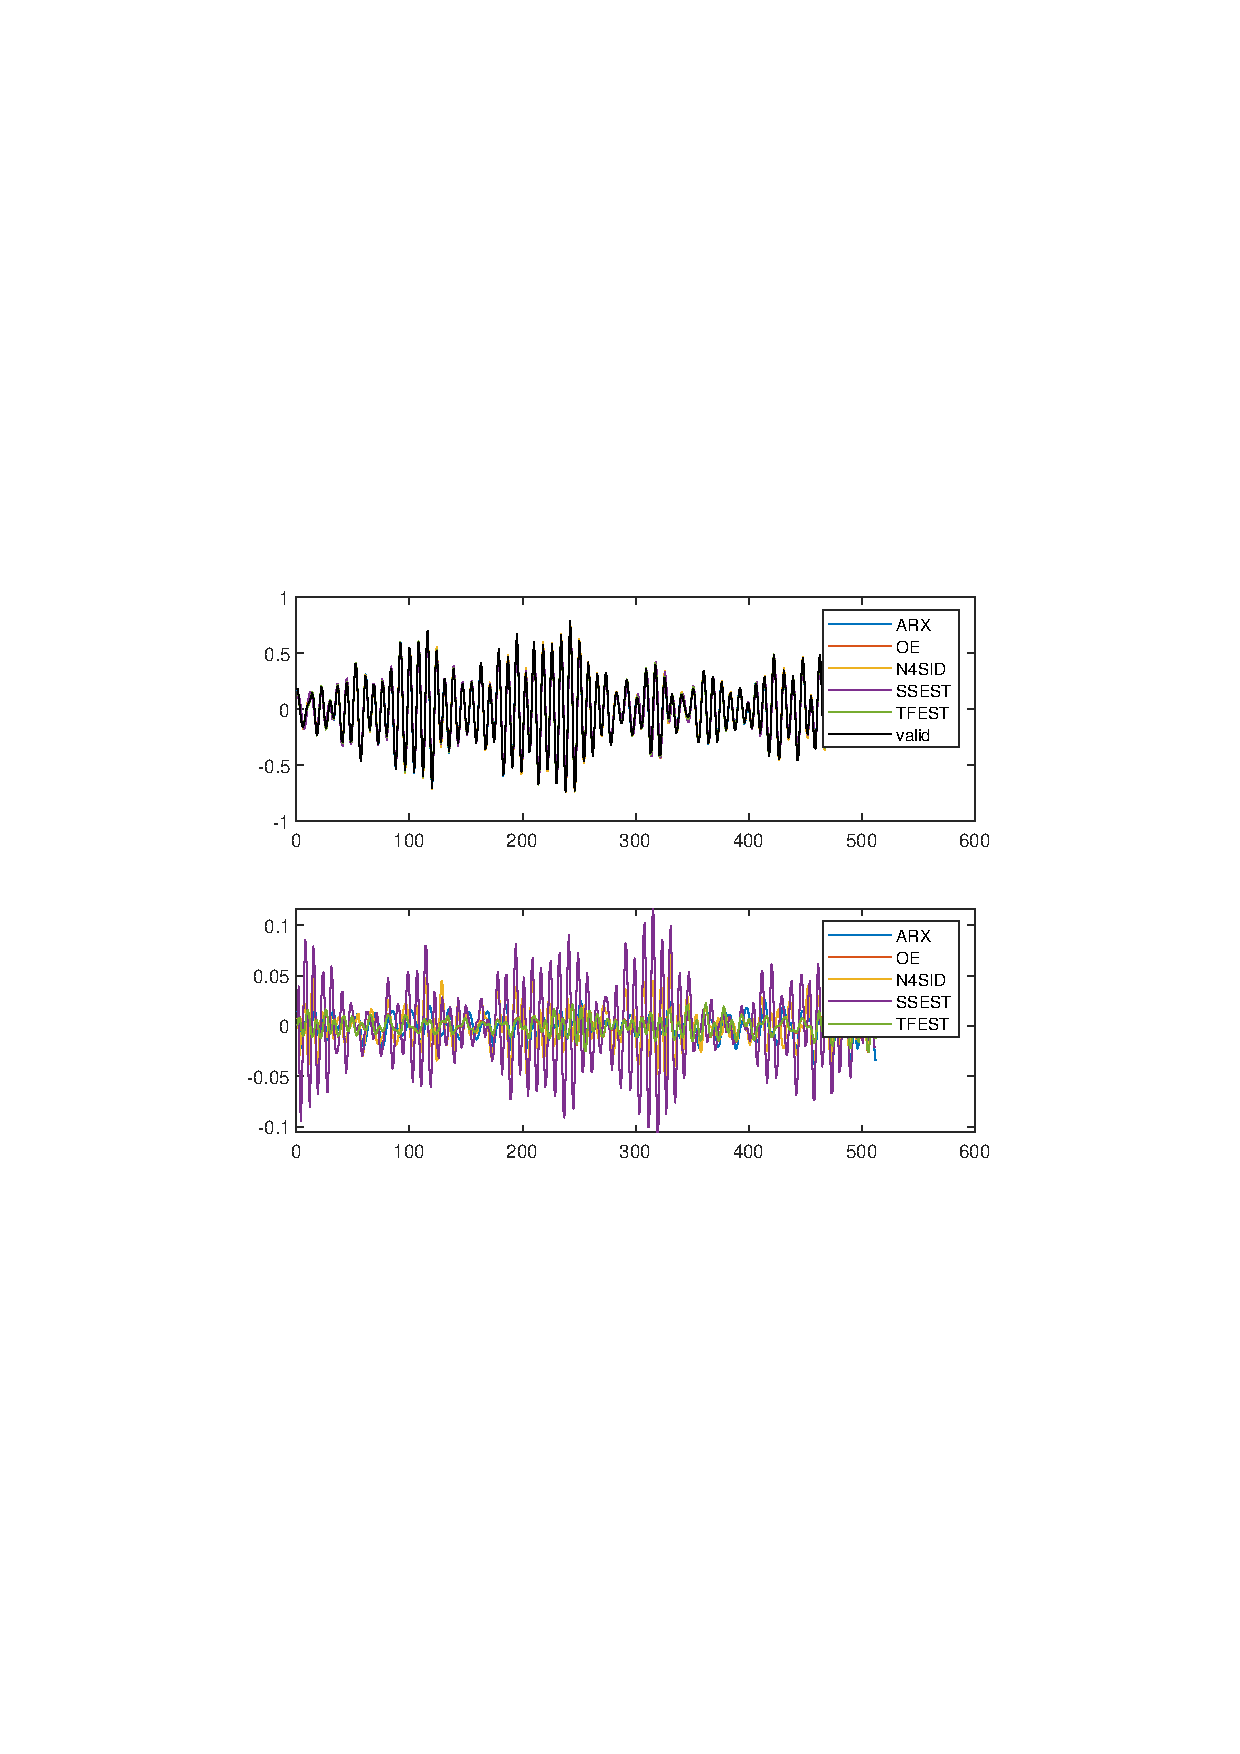
\includegraphics[trim= 10cm 8cm 10cm 8cm, scale=0.4]{figures/simulations.pdf}
\end{subfigure}
\begin{subfigure}{.49\textwidth}
	\centering
	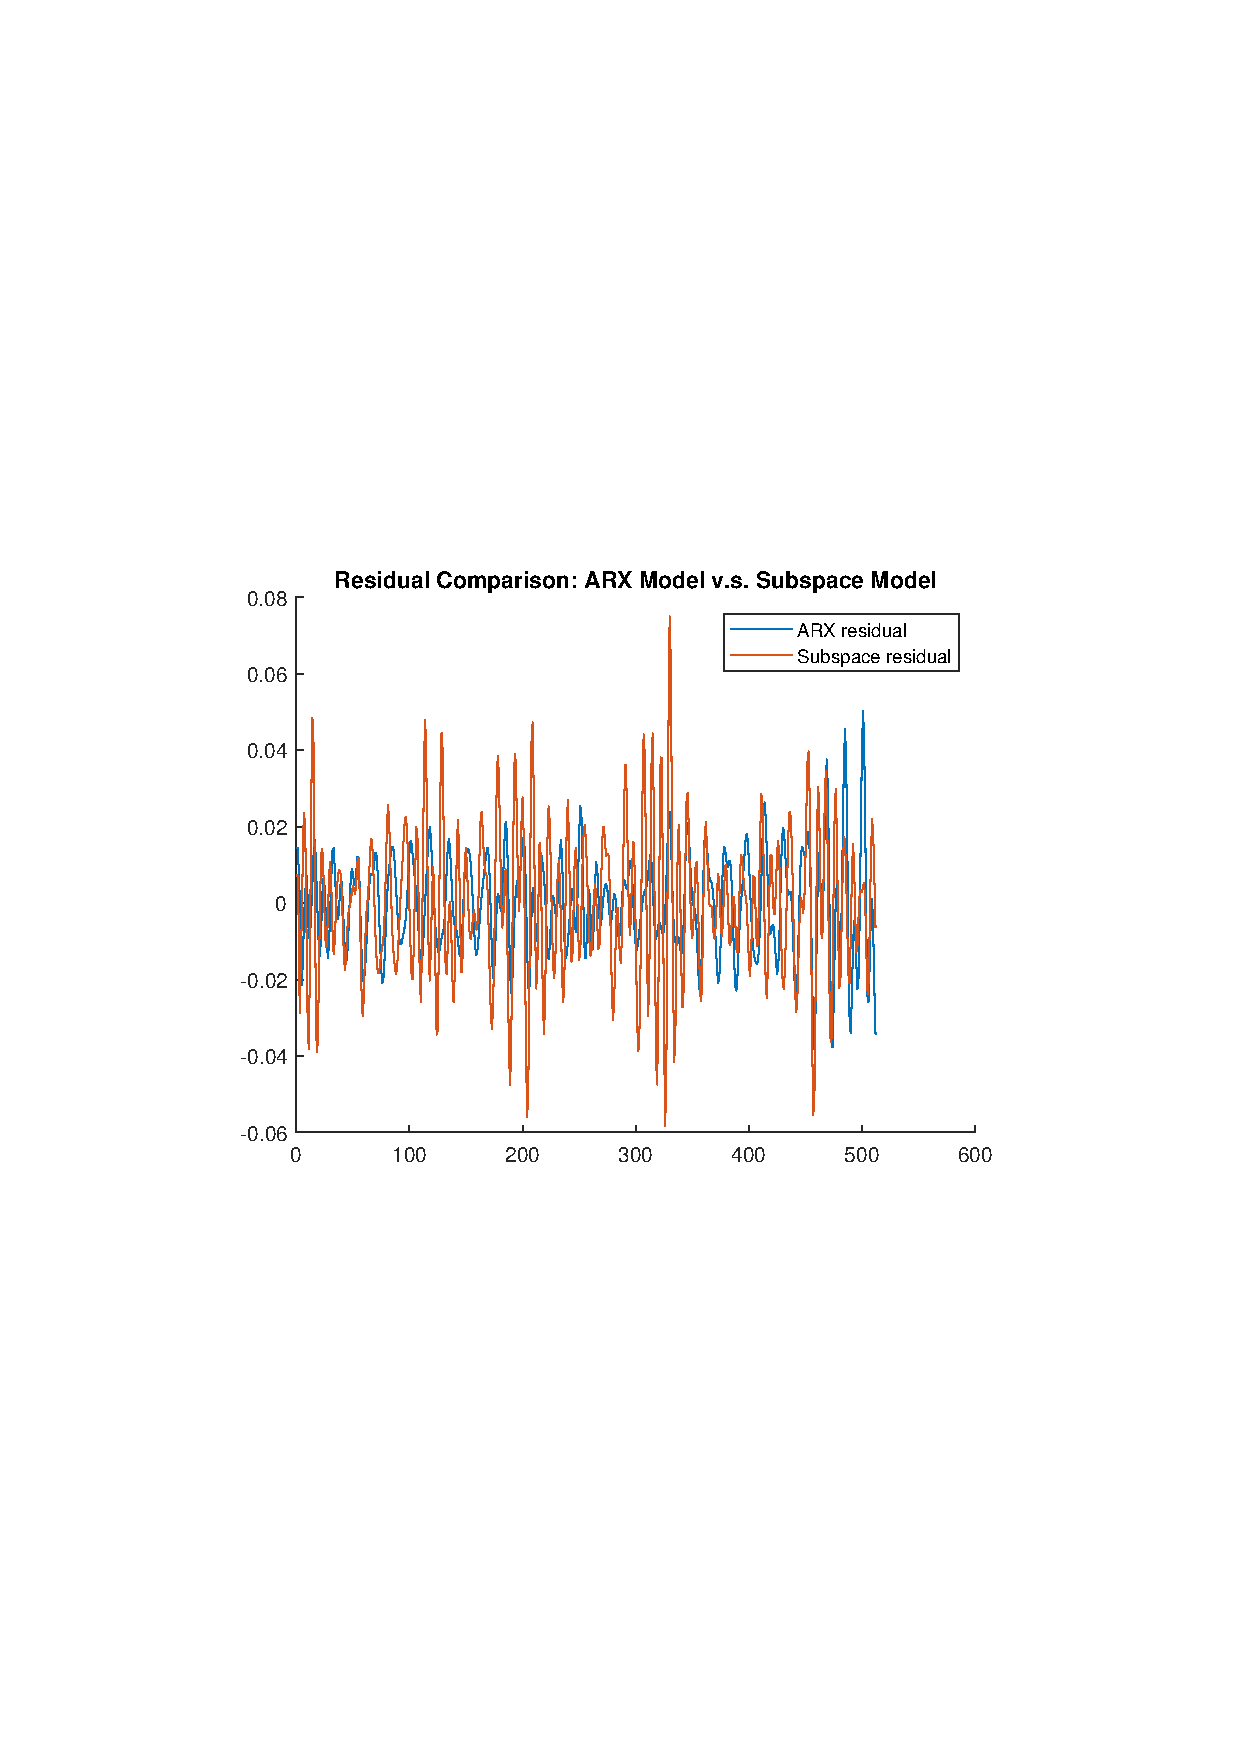
\includegraphics[trim= 10cm 8cm 10cm 8cm, scale=0.4]{figures/sim_diff_arx_ss.pdf}
\end{subfigure}
\caption{Simulations (left) and simulation error comparison of ARX and State Space model (right).}
\label{fig:simulations}
\end{figure}

\begin{figure}[ht]
\centering
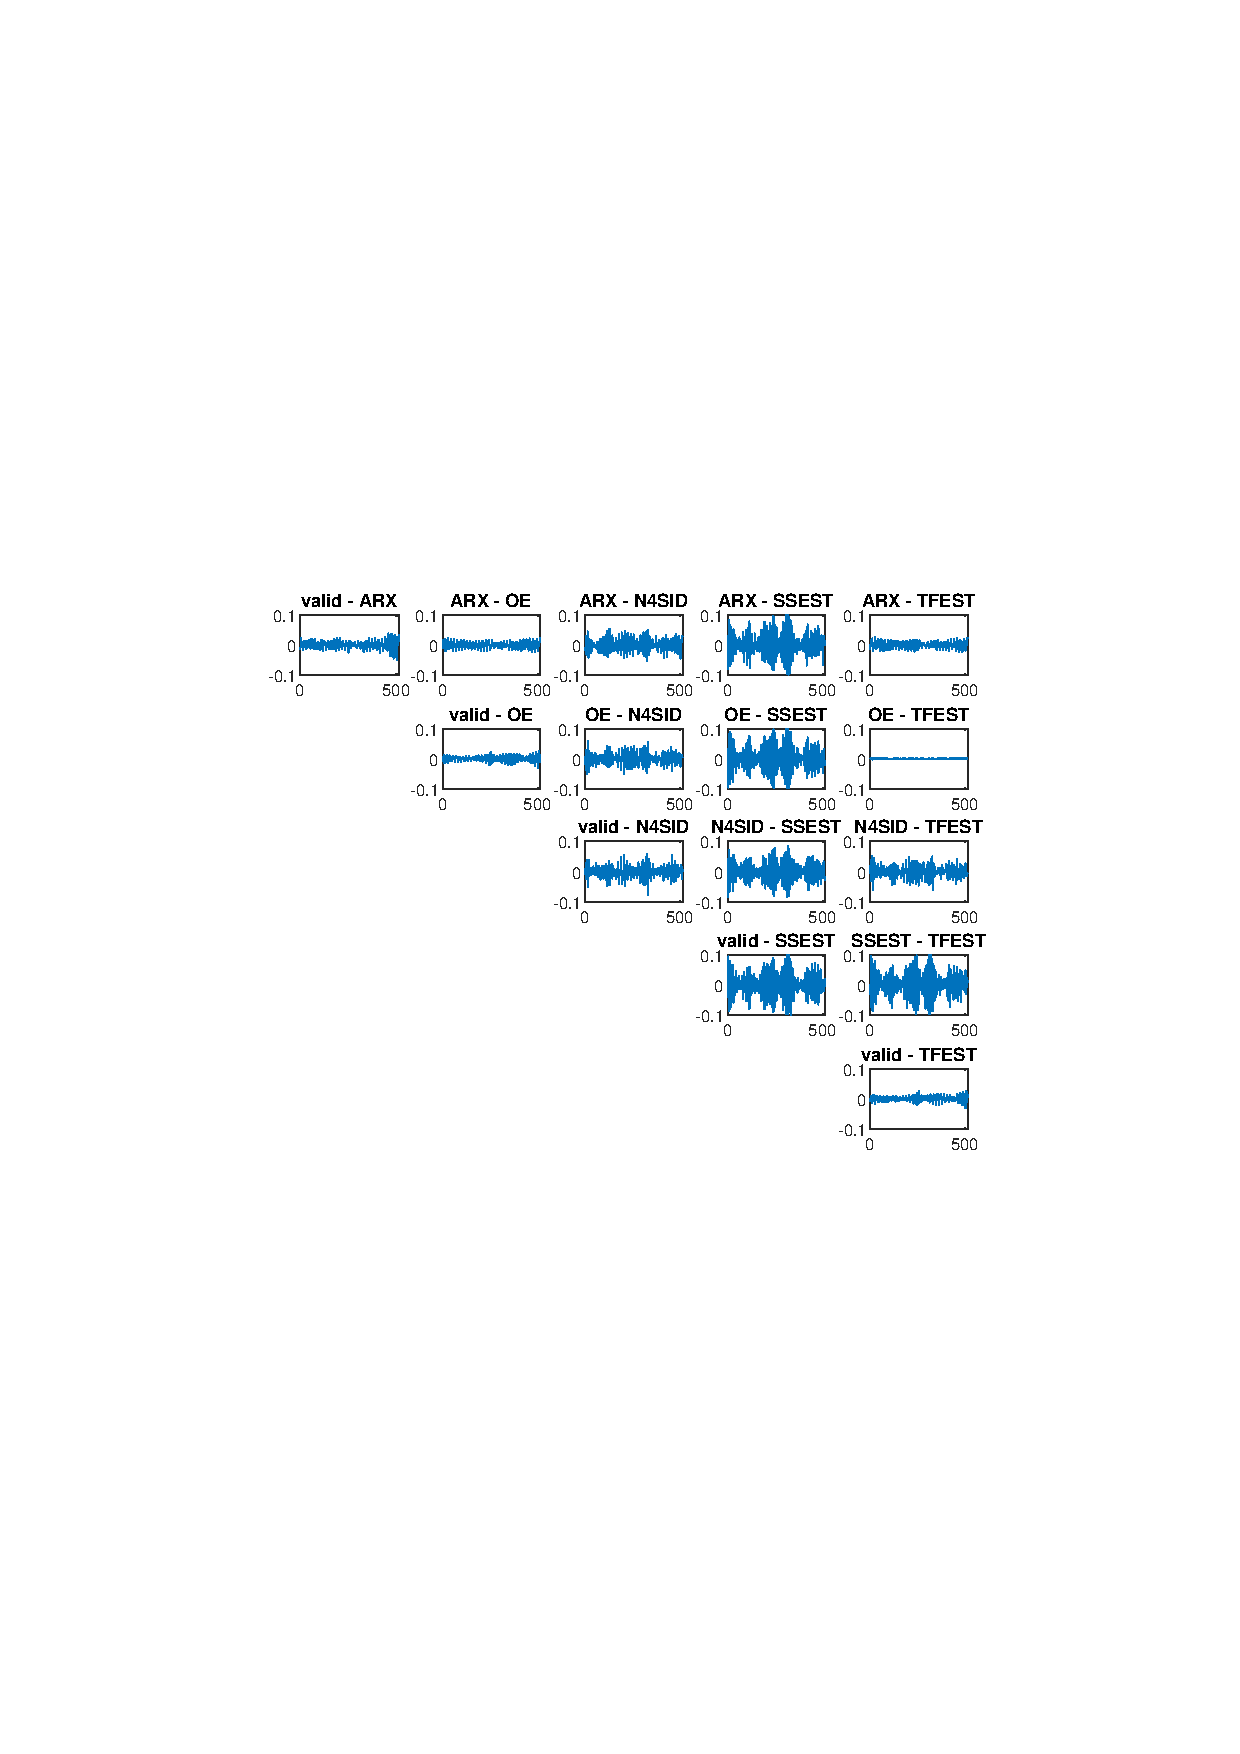
\includegraphics[trim= 10cm 8cm 10cm 8cm, scale=0.7]{figures/sim_diff_matrix.pdf}
\caption{Model differences and simulation vs validation data error on diagonal.}
\label{fig:model_differences_simulation}
\end{figure}

In the left plot of Figure \ref{fig:simulations} shows the simulation error of different models. Here, it is obvious to see that for the state space model estimated using prediction error method has the worst performance. Figure \ref{fig:model_differences_simulation} shows the comparison of different models. For the plots on the diagonal, the simulated output is compared to true data. We can see that the OE model and the transfer function model are very similar. It is due to the fact that the only difference between these two models is that for the transfer function model, there is a feedthrough option that allows us to choose b0 in the numerator, while b0 is always zero in the OE model. Figure shows that the ARX model has less simulation error. 

\paragraph{Predictions}

\begin{figure}[ht]
\centering
\begin{subfigure}{.49\textwidth}
	\centering
	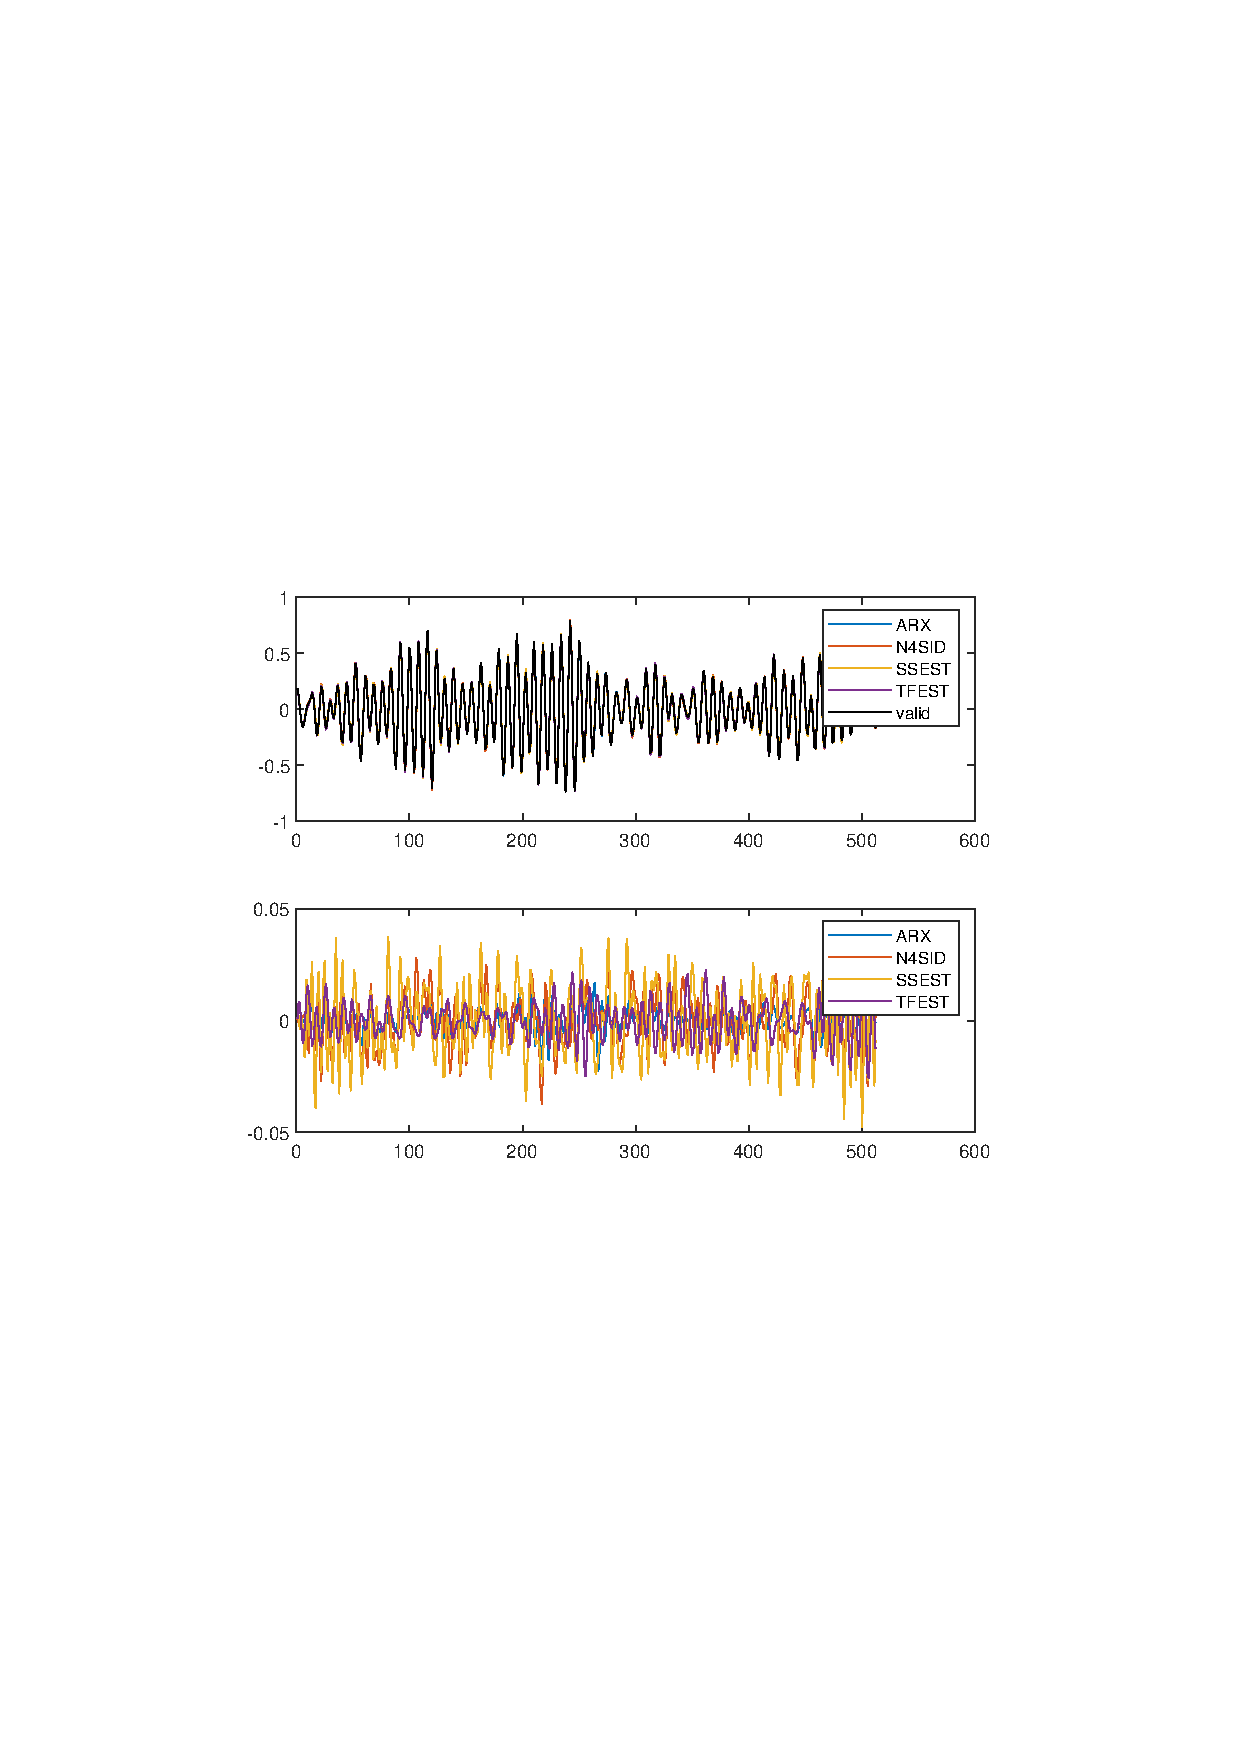
\includegraphics[trim= 10cm 8cm 10cm 8cm, scale=0.4]{figures/predictions.pdf}
\end{subfigure}
\begin{subfigure}{.49\textwidth}
	\centering
	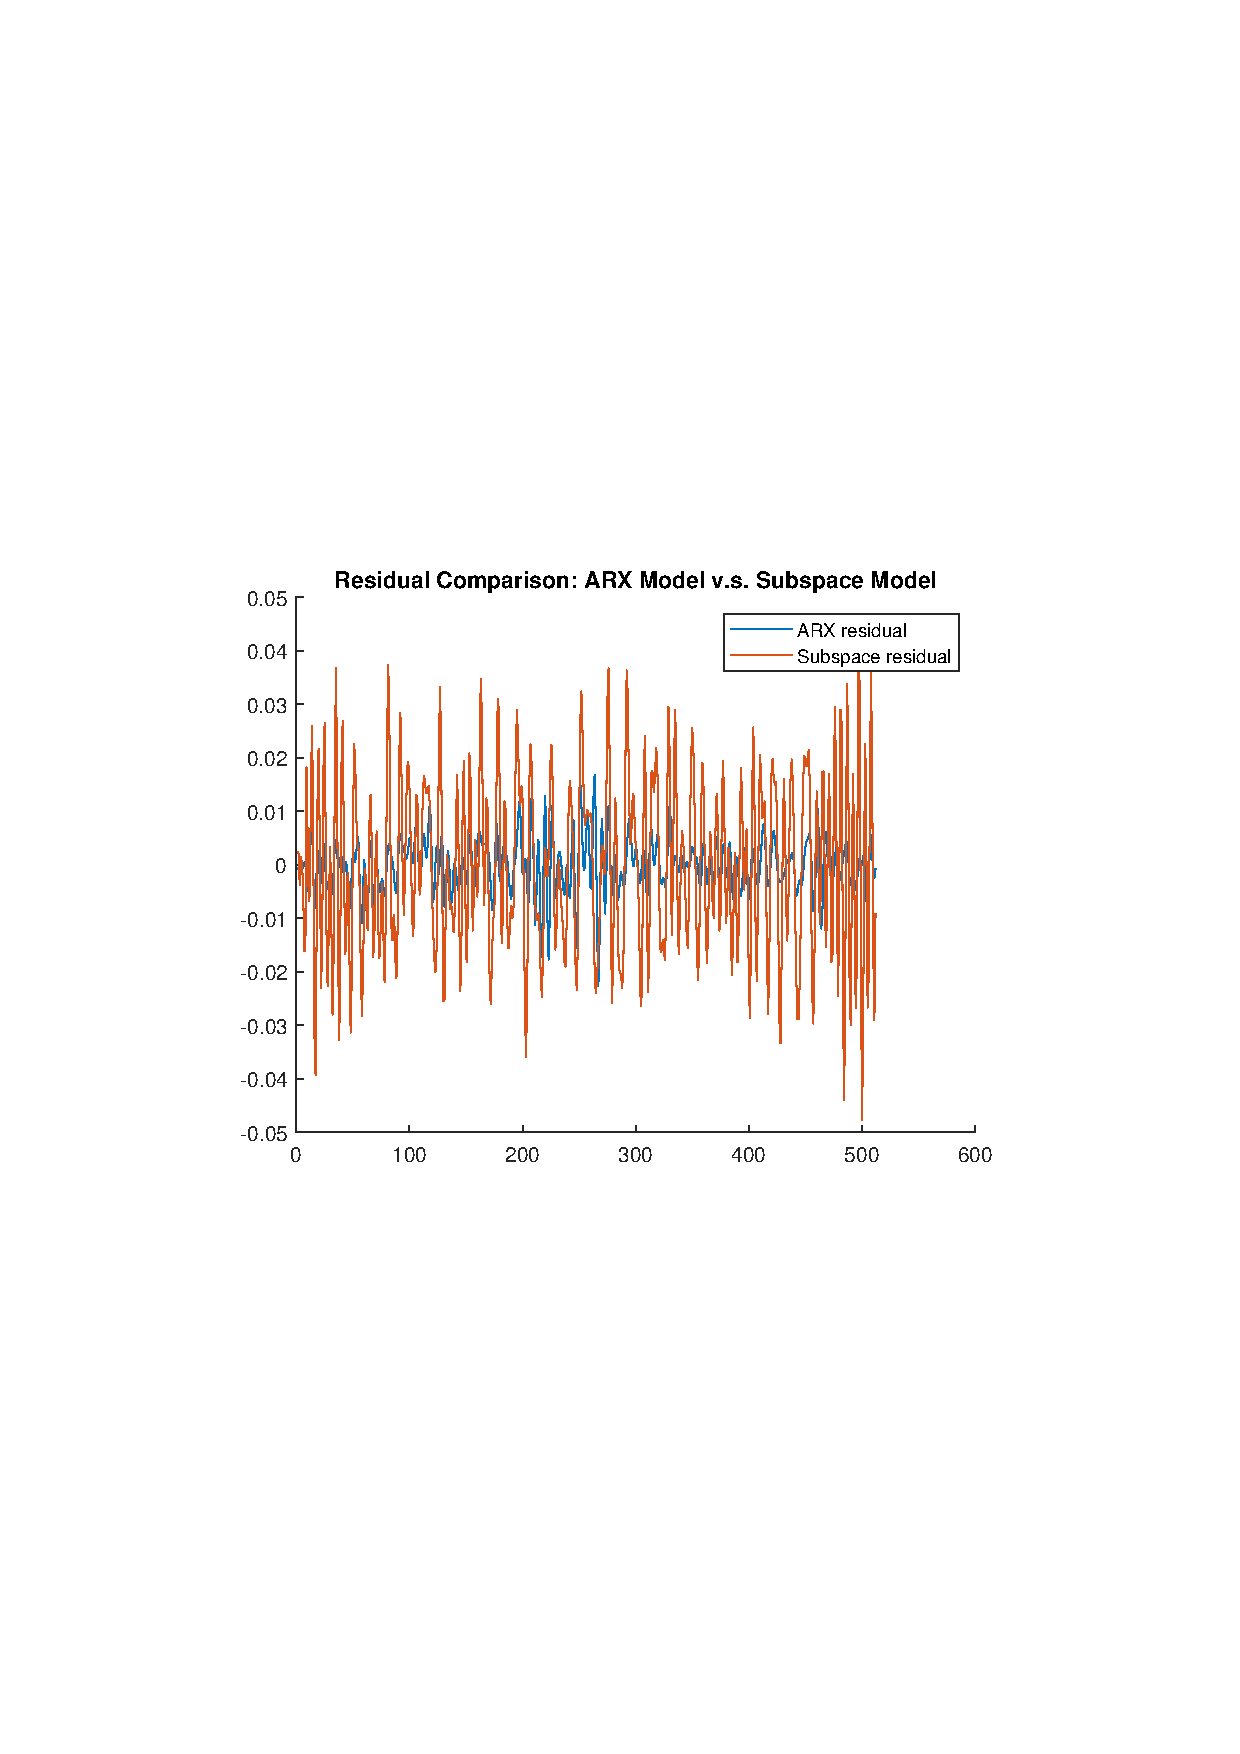
\includegraphics[trim= 10cm 8cm 10cm 8cm, scale=0.4]{figures/pred_diff_arx_ss.pdf}
\end{subfigure}
\caption{Predictions (left) and prediction error comparison of ARX and State Space model (right).}
\label{fig:predictions}
\end{figure}

\begin{figure}[ht]
\centering
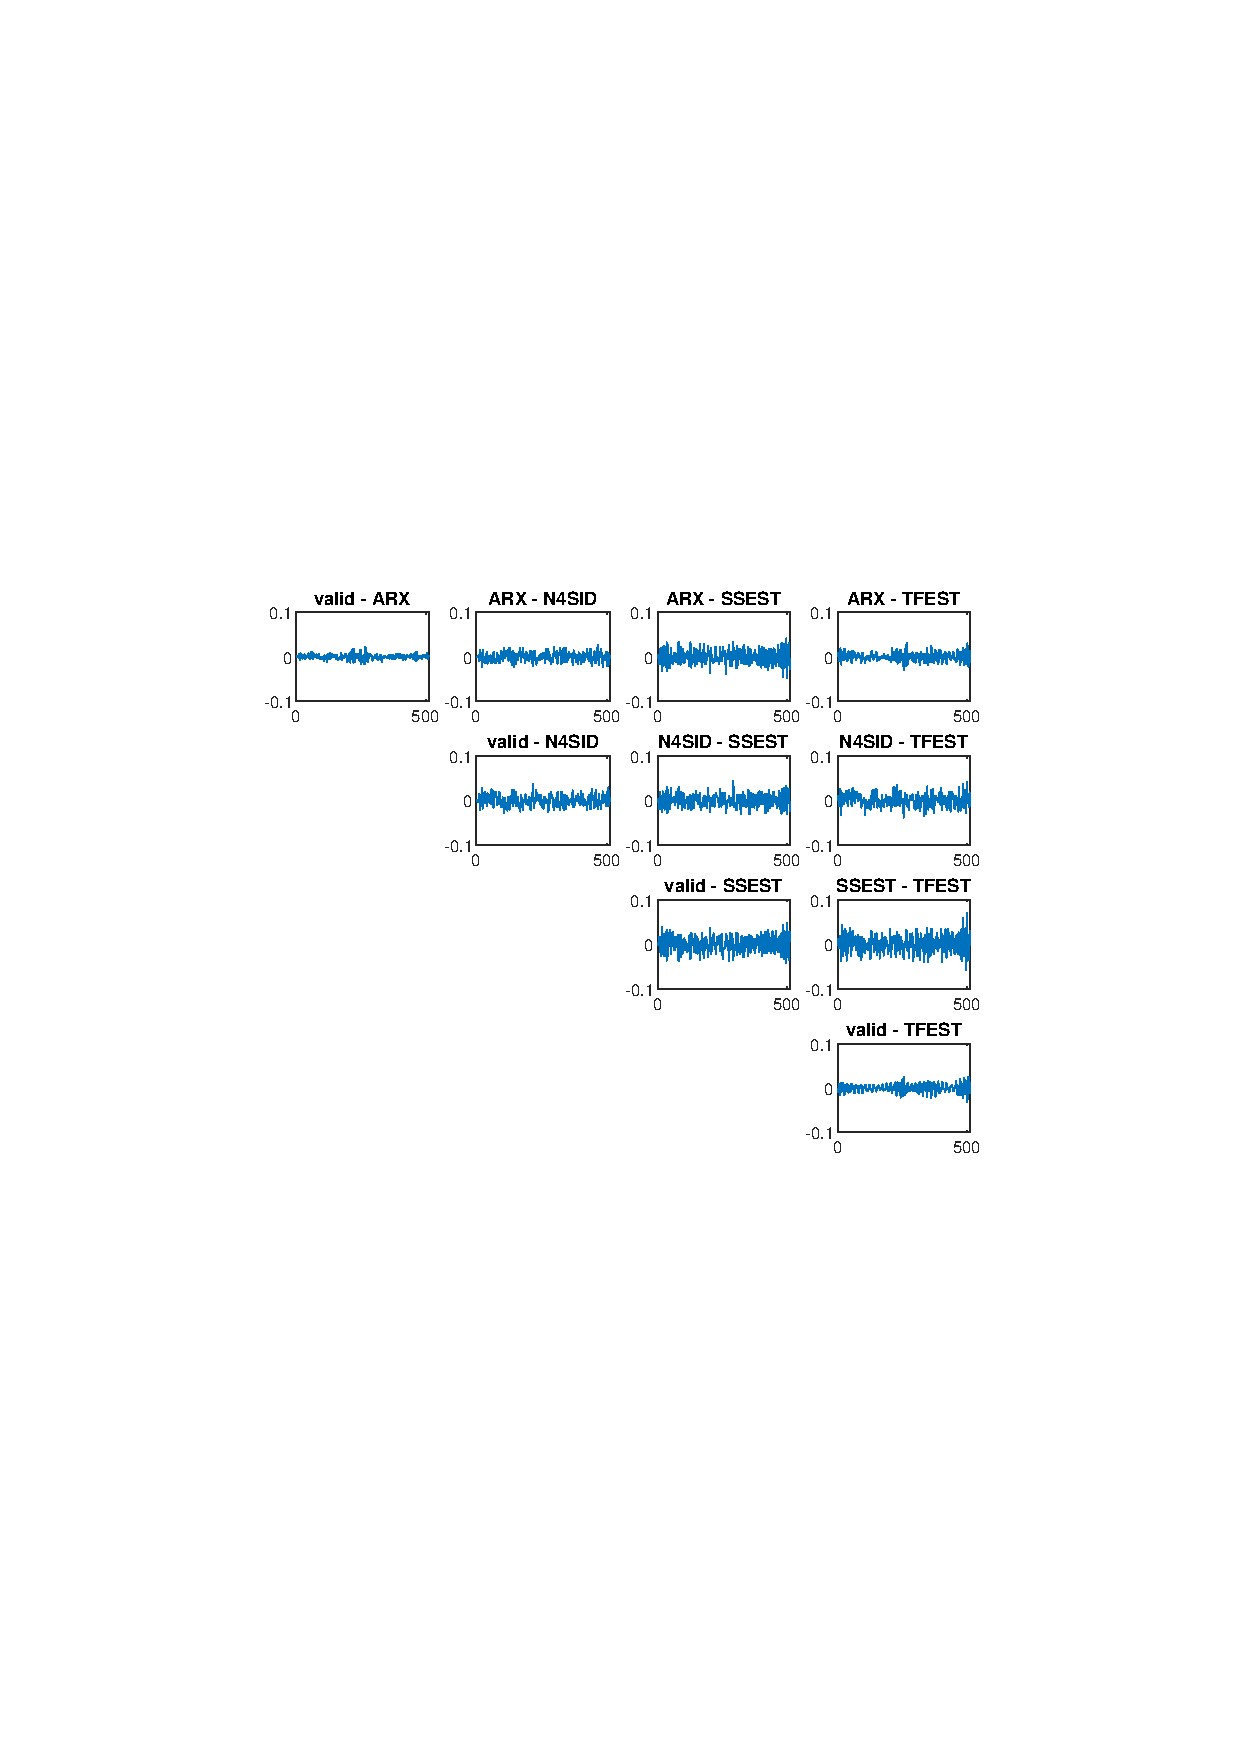
\includegraphics[trim= 10cm 8cm 10cm 8cm, scale=0.7]{figures/pred_diff_matrix.pdf}
\caption{Model differences and prediction vs validation data error on diagonal.}
\label{fig:model_differences_prediction}
\end{figure}

\paragraph{Correlations}
\begin{figure}[ht]
\centering
\begin{subfigure}{.49\textwidth}
	\centering
	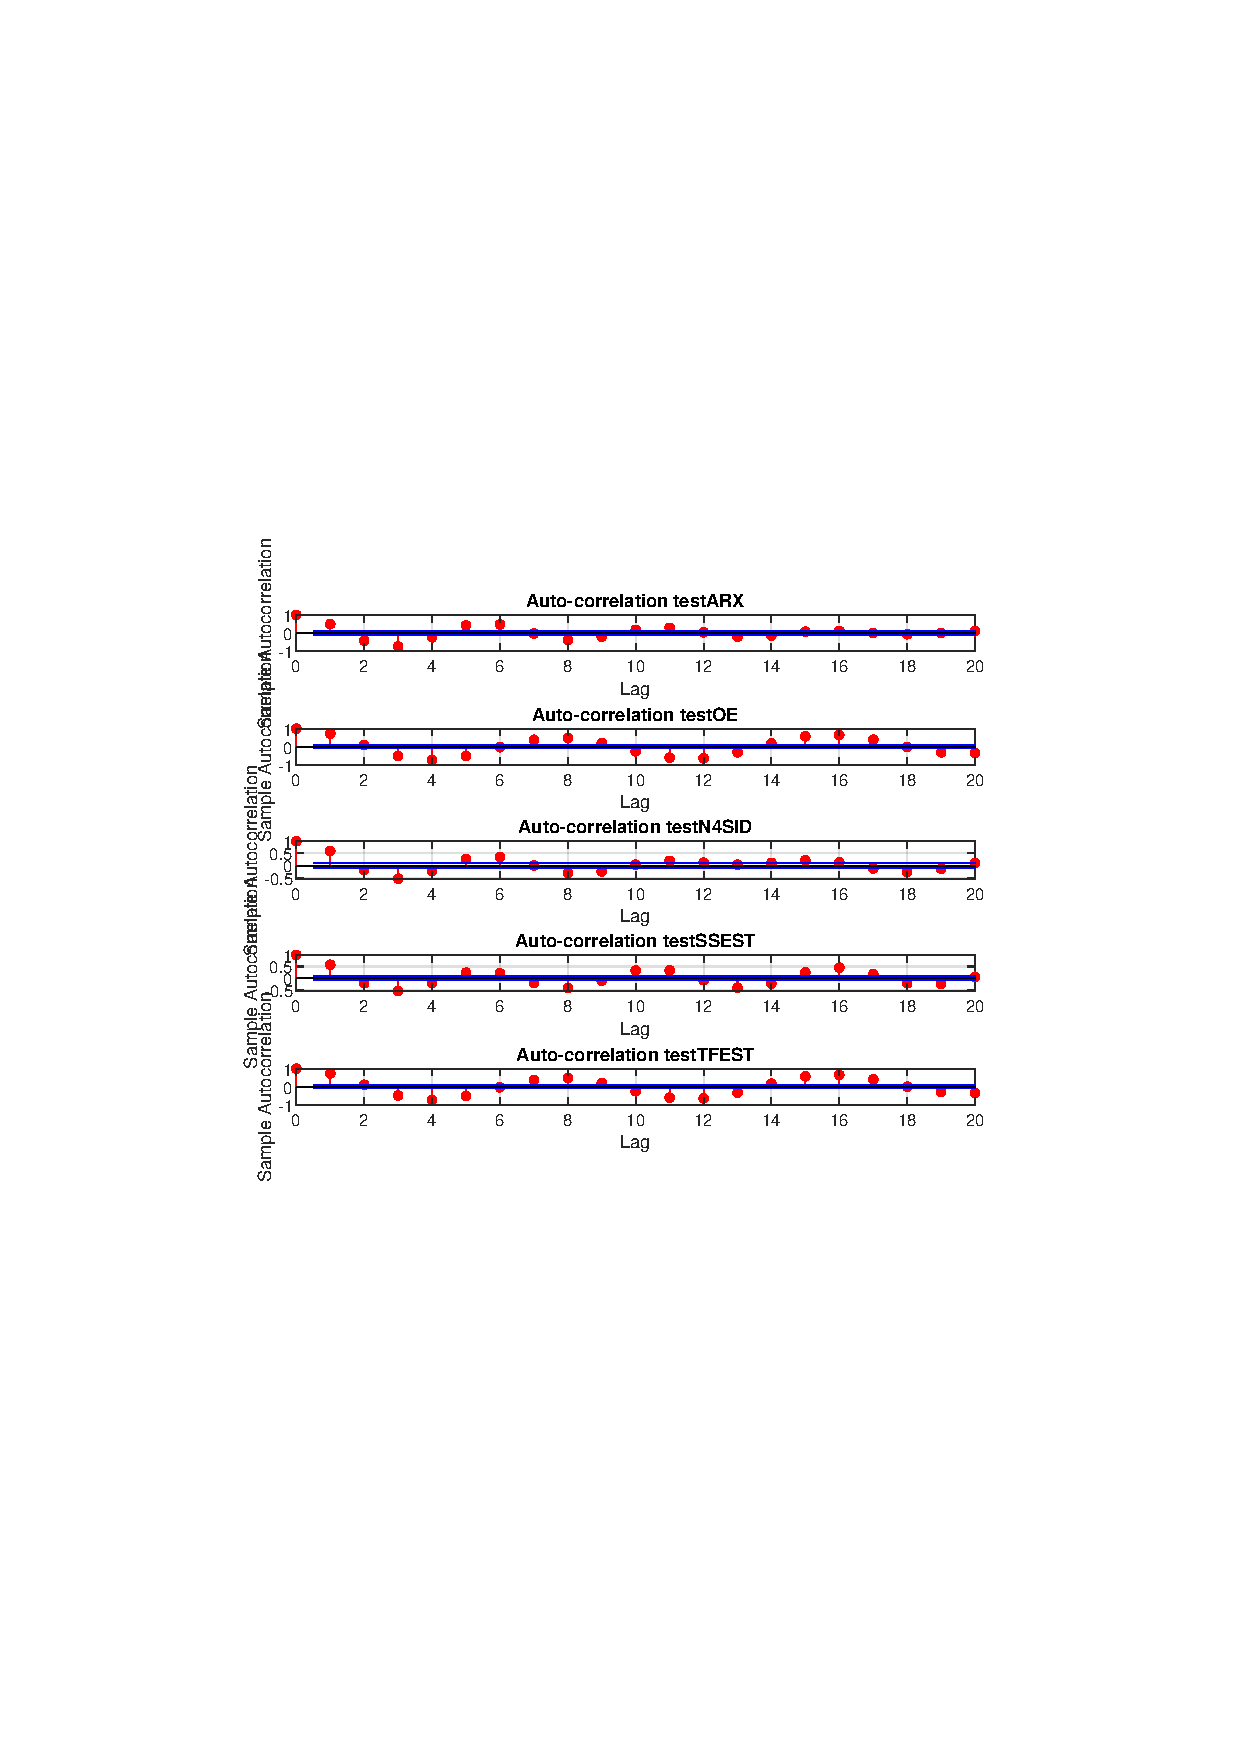
\includegraphics[trim= 10cm 8cm 10cm 8cm, scale=0.4]{figures/auto-corr-1step.pdf}
\end{subfigure}
\begin{subfigure}{.49\textwidth}
	\centering
	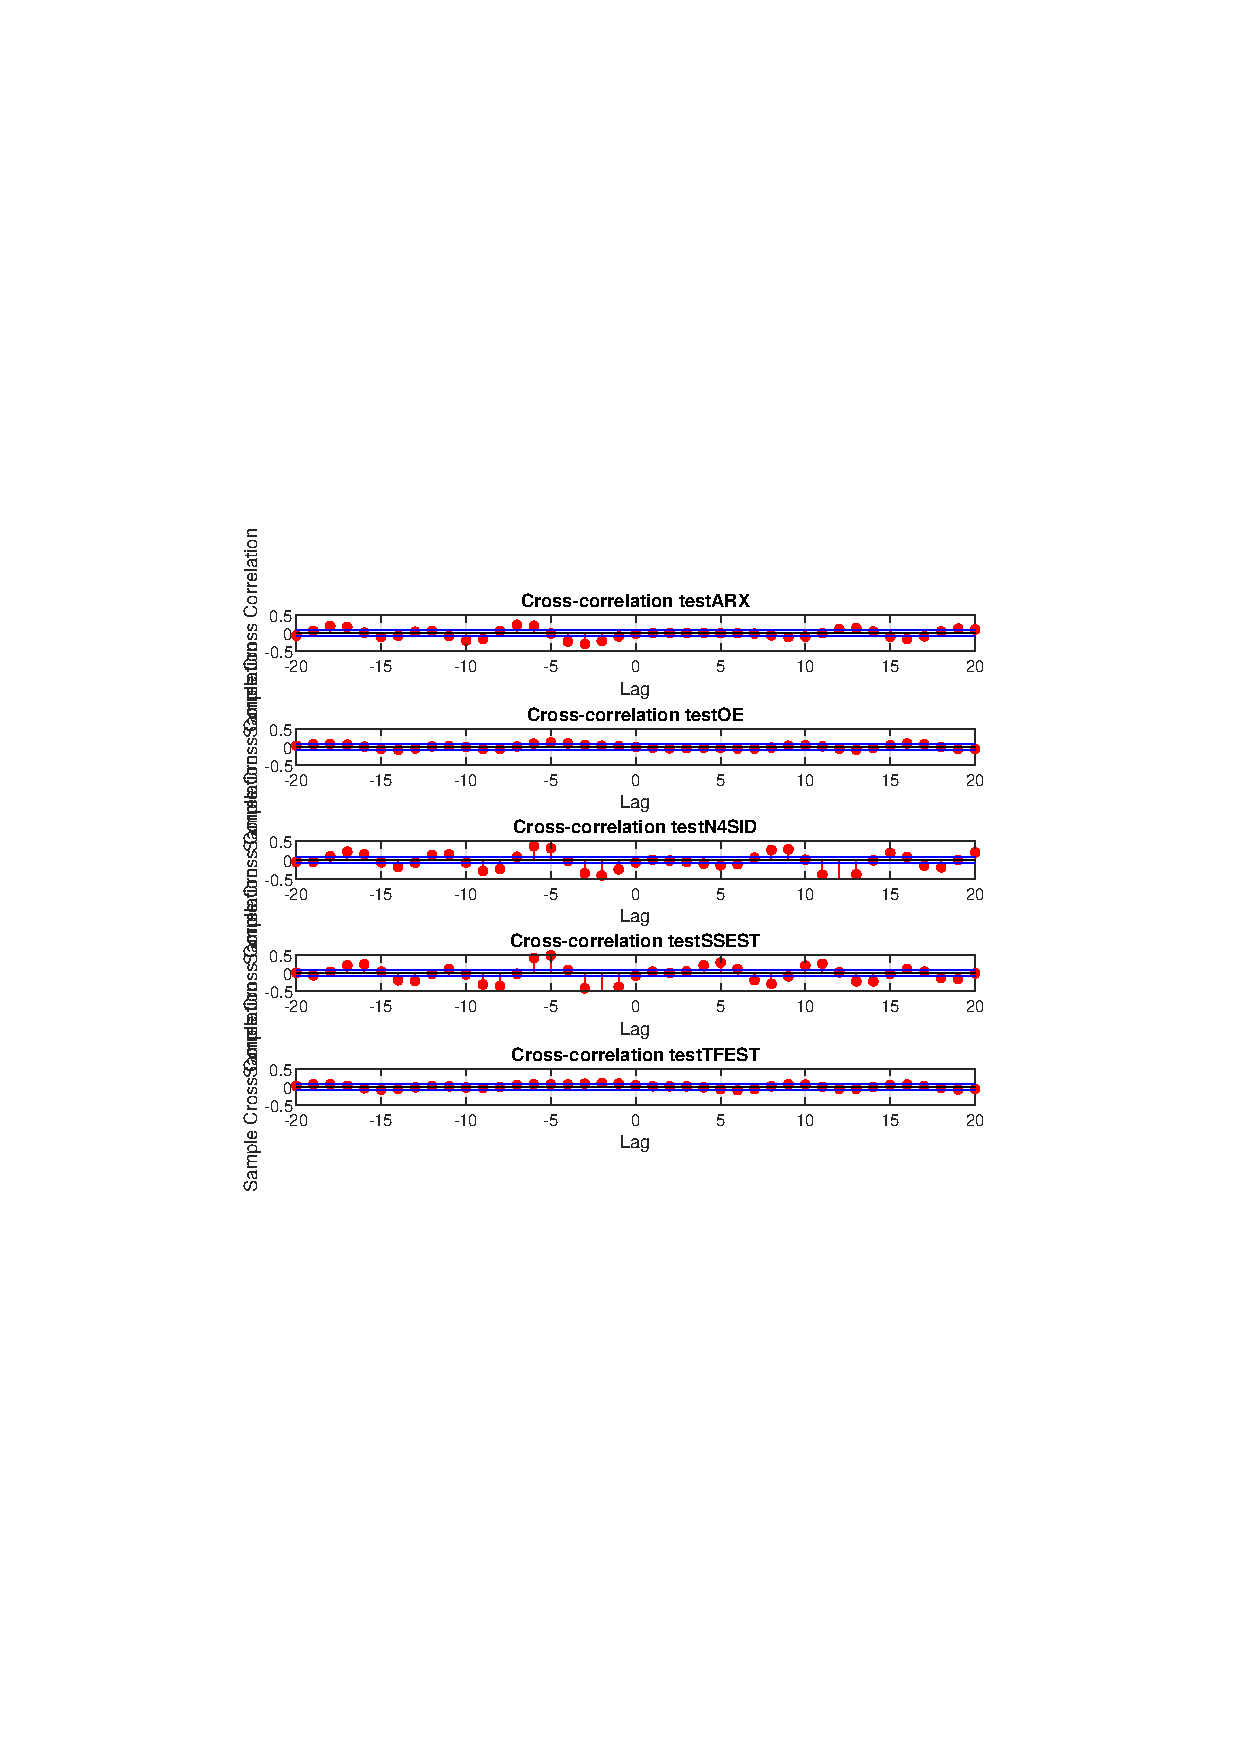
\includegraphics[trim= 10cm 8cm 10cm 8cm, scale=0.4]{figures/cross-corr-1step.pdf}
\end{subfigure}
\caption{Auto-Correlation (left) and cross-correlation (right).}
\label{fig:correlations}
\end{figure}

Next, we did the residual analysis regarding its autocorrelation and its cross-correlation with the input. For a perfect-fitting model, the auto or cross correlation with the input should be zero expect when the lag is zero. In Figure \ref{fig:correlations}, we can see that the ARX model and the state space model estimated using subspace method are better than the rests. However, from this cross-correlation plot, we can see that the state space model is not very good due to the correlation is not zero when the lag is large and that the normalised magnetite also often exceeds the 95% confidence region. Overall, the ARX model is the best. 

\subsubsection{Non-linear models}

In this subsection, we compare the linear model with several non-linear models regarding 5-step prediction error and simulation error in the terms of fitting rate, which is calculated as
\begin{equation}
	fit\% = (1-\frac{\sum(y(t)-\hat{y}(t))^2}{\sum(y(t)-\bar{y})^2})*100.
\end{equation}

\begin{figure}[ht]
\centering
\begin{subfigure}{.49\textwidth}
	\centering
	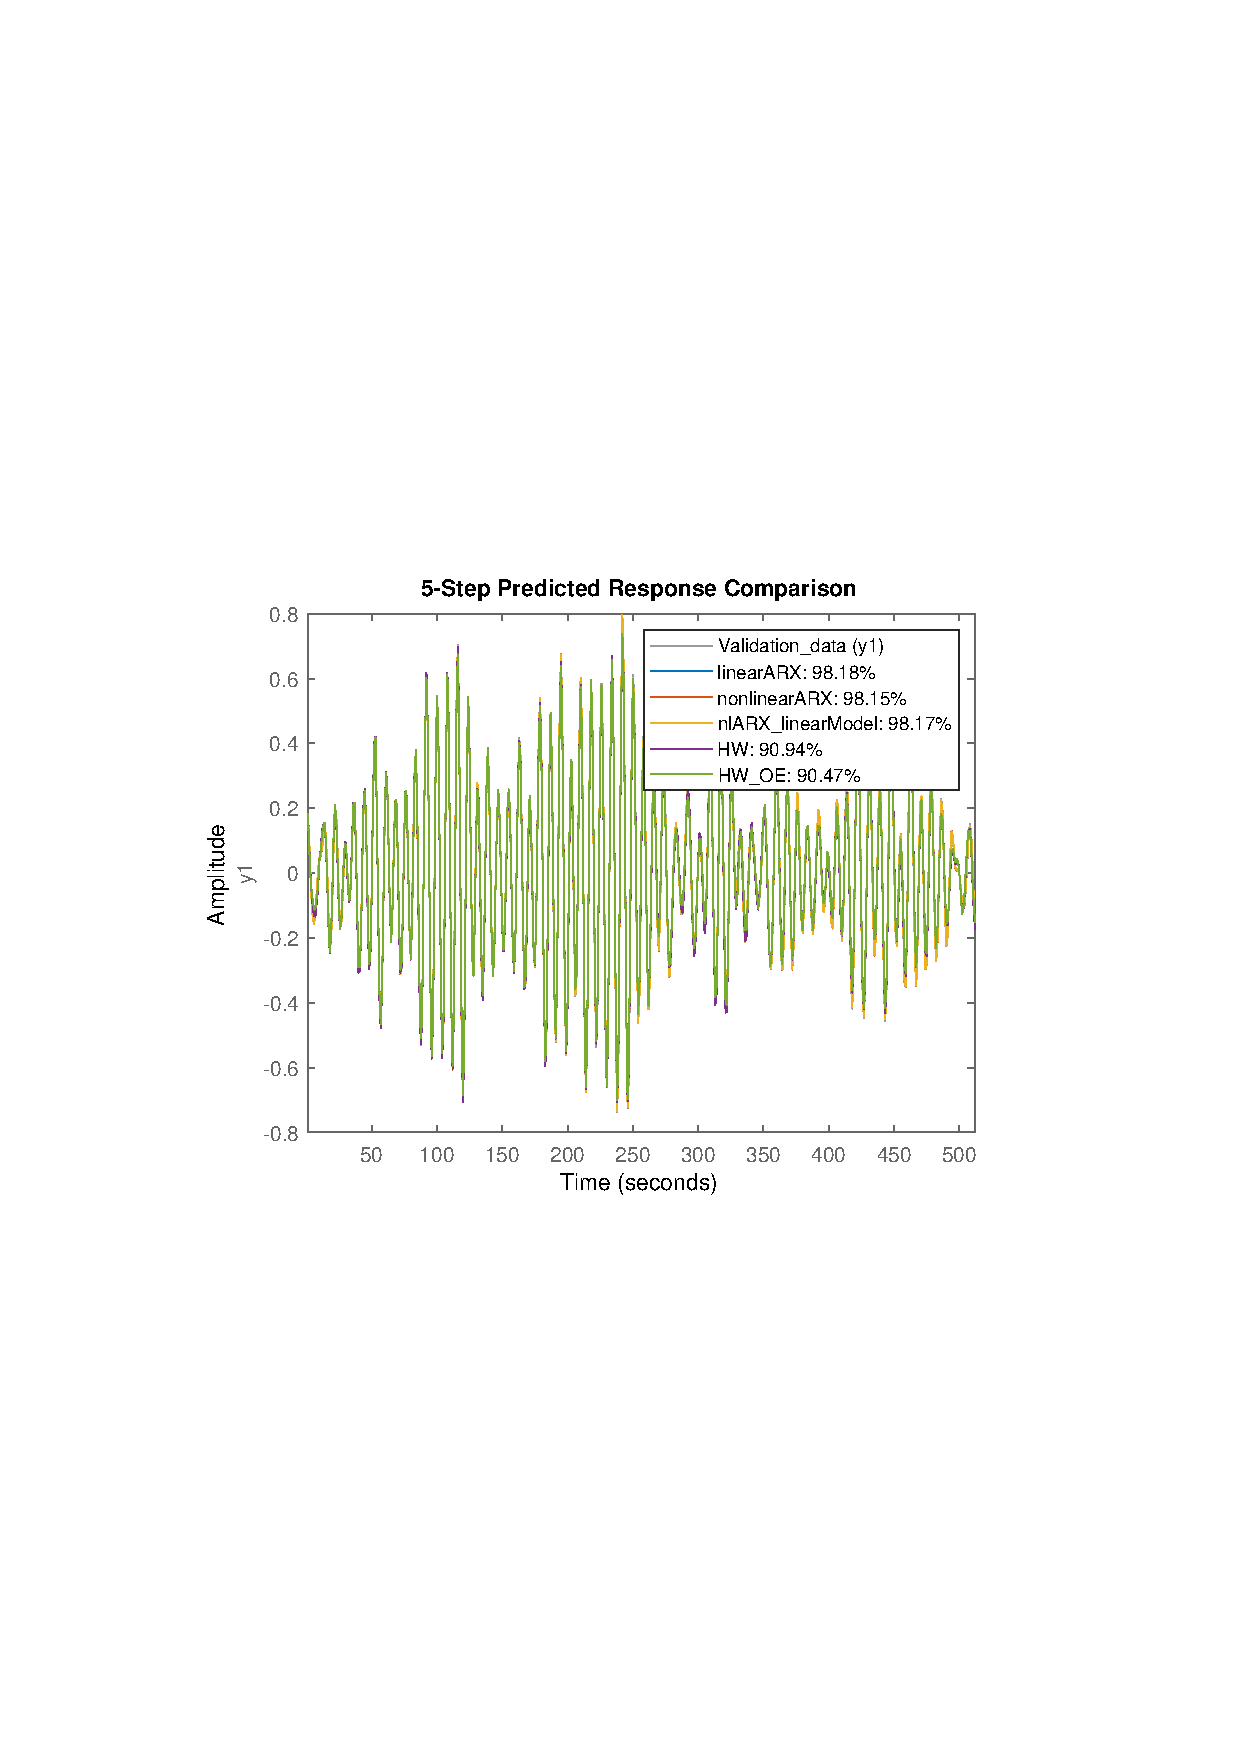
\includegraphics[trim= 10cm 8cm 10cm 8cm, scale=0.4]{figures/predictions_nl.pdf}
\end{subfigure}
\begin{subfigure}{.49\textwidth}
	\centering
	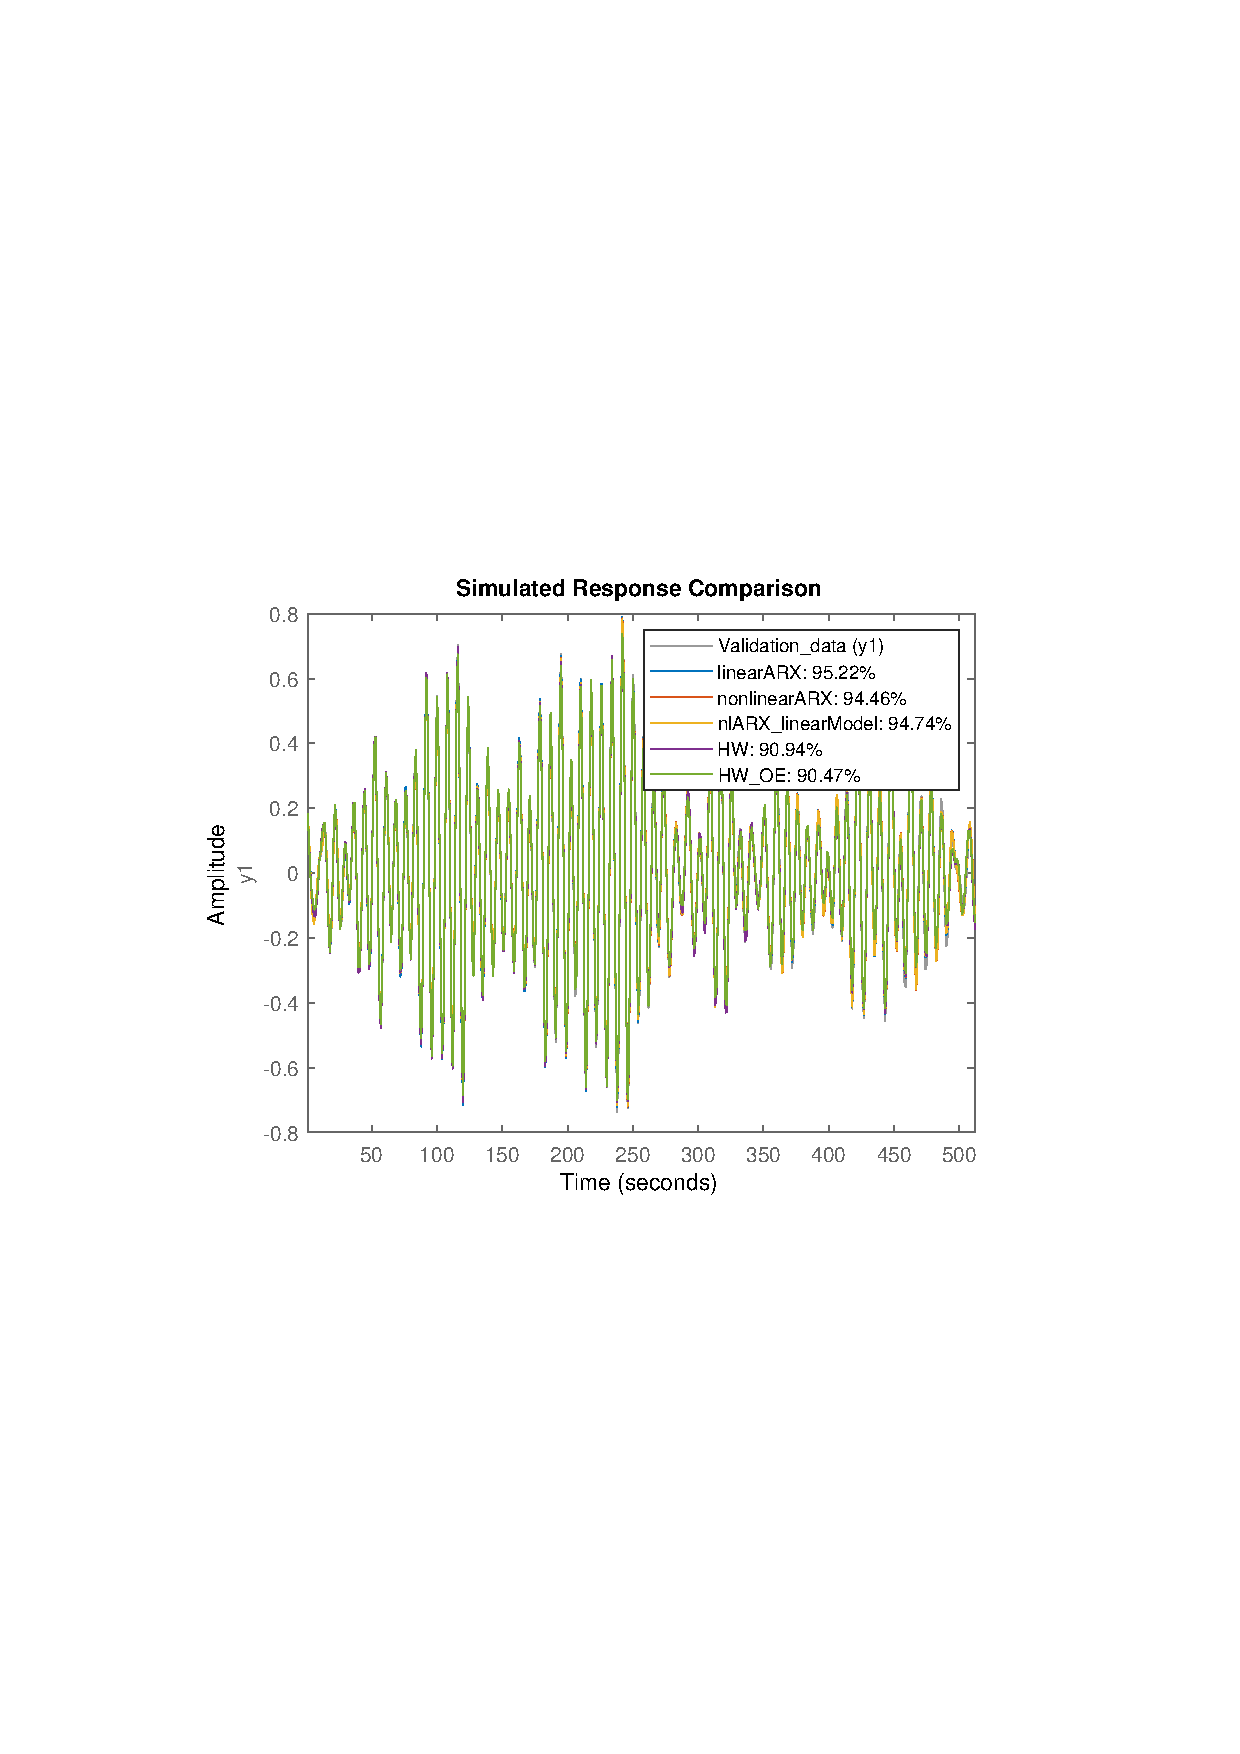
\includegraphics[trim= 10cm 8cm 10cm 8cm, scale=0.4]{figures/simulations_nl.pdf}
\end{subfigure}
\caption{Non-linear model predictions (left) and simulations (right).}
\label{fig:nonlinear}
\end{figure}

It can be seen from Figure \ref{fig:nonlinear} that the non-linear models estimated using the non-linear ARX model has higher fitting rate than those identified using the non-linear Hammerstein-Wiener model. For a non-linear model, it can be estimated either by directly using the estimated data or by adding non-linearity to an identified linear model for refinement. However, in our case, when we estimated the default non-linear model using an input-output polynomial model of ARX or OE structure, the fitting rate did not increase compared to the result directly estimated using the linear model. Thus, we can draw the conclusion that there is little or no non-linearity in our data.

We also did some non-linear identification on our data. If we can obtain better performance using nonlinear model, then we can say that there are some non-linearities existing in our model. We tried the non-linear ARX model and the Hammerstein-Wiener model. Hammerstein-Wiener models describe dynamic systems using one or two static nonlinear blocks in series with a linear OE block, whereas in the non-linear ARX model, the regressors are followed by a non-linearity block. For the non-linear models, we can either choose to use the default option or we can initialize the non-linear system identification with an identified linear model, which means that the we start the model estimation with the linear model and begin the search by adding some non-linearities. However, from this figure we can see that, adding non-linearities to the linear model does not improve the model fitting rate. From this, we can infer that there is little or no non-linearity in the true model. 


\end{document}
